

\chapter{Signal Optimization}


After the preselection, additional selection criteria is performed to optimize the discrimination power for a Higgs signal.

\section{Tagging Classification}

Once the events are preselected as described in the previous sections, they are classified according to the b-tagging (see section~\ref{subsec:btaggingofjets})  of the jets associated to the Higgs candidate. Events are classified as ``two tags'' if the two jets are b-tagged with at least one medium-tag and one loose-tag. Events failing that requirement are classified as ``one tag'' if at least one of the two jets satisfy the loose-tag condition. Events failing this requirement are finally classified as ``no-tag''.  These three categories are mutually exclusive.  A summary can be seen in Table~\ref{tab:btagcateg}.

%%%%%%%%%%%%%%%%%%%%%%%%%%%%%%%%
\begin{table*}[htb!]
\caption{ 
B-tag categories.
}
\label{tab:btagcateg}
\vspace*{\medskipamount}
\begin{center}
\small
\begin{tabular}{|c|c|}
\hline
Tag Region & Description\\
\hline
0-tag & jet is not tagged Loose; other jet is not tagged Loose \\
1-tag & jet is tagged Loose; other jet is not tagged Medium \\
2-tag & jet is tagged Medium; other jet is tagged Loose \\
\hline
\end{tabular}
\end{center}
\end{table*}
%%%%%%%%%%%%%%%%%%%%%%%%%%%%%%%%%%%%%%%%%%%%%%%%%

As these three categories present very different signal-to-background ratios they are treated separately in the final optimization. In addition, some differences in the selection are also needed due to the different background composition, especially in the case of the ``two tags'' sample, in which the $t\overline{t}$ background starts to be noticeable. On the other hand, since the optimization is based mostly on the intrinsic properties of the final state under investigation, there are analysis strategies that are shared by the three categories. The main differences between the categories are that the 2 b-tag category has the highest purity, but has very low signal yield.  Opposed to that, the 0 b-tag category has the largest signal yield but is dominated by Z+jets background. The 1 b-tag category is affected by both issues and therefore has the least discriminating power.

There are differences in the b-tagging between data and those predicted by Monte Carlo.  These differences are corrected by b-tagging scale factors.  These are used to adjust two different problems.  The first is the efficiency that the JP algorithm will not recognize a b-jet even if it is from a heavy flavored quark.  Second, the light quarks or gluons are incorrectly identified as b-jets.  

The efficiency ($SF_{hf}$) (from non tagging of heavy quarks) and the mis-identification rate ($SF_{lf}$) (labeling light quarks and gluons as b-jets) are defined as the ratio of tagging efficiency between heavy and light flavor jets in data and simulations.  These are typically functions of $p_T$ and the pseudo-rapidity of the jets.  Typically $SF_{hf}$ is smaller than one because in data the successful tagging of heavy quarks is better than in simulation.  Oppositely, $SF_{lf}$ is typically larger than one because tagging light quarks in data as b-jets is more common than in simulation.  In general all jets, regardless of flavor, are tagged as b-jets more frequently in data than jets in simulation~\cite{CMS-PAS-BTV-11-004}.

The b-tagging performance is corrected between data and simulation, but we must take additional steps than simply scaling the JP distribution.  This is because our classification of events is based on the jet flavor of both tagged and non-tagged jets.  The process to correctly distribute candidates between the categories is as follows.  As the scale factors change the jets momentum there is a percentage of jets that would migrate to a different b-tagged category. Using a random number generator candidates are upgraded or downgraded between the different b-tagging categories according to the scale factor percentages. This gives jets that are tagged a non zero chance of being lowered to another category or non-tagged jets to be raised to a higher category.  For example, a medium-tagged jet can be lowered to a loose-tagged jet, or a loose-tagged jet can be lowered to a non-tagged jet.  Also, a non-tagged jet can be promoted to a loose-tagged jet, or a loose-tagged jet can be promoted to a medium-tagged jet~\cite{2l2q115}.


\section{Helicity Likelihood}

There are a number of kinematic differences between the $H \rightarrow ZZ \rightarrow 2l2q$ decay and the Z + jets background.  When a heavy Higgs boson is produced and decays into two Z bosons, those Z bosons have boosted kinematics.  The $p_T$ of the Z bosons increases with the mass of the parent particle, the Higgs boson.  Another powerful variable to separate signal from background is the $\Delta R$ spacing between the two jets, leptons, and Z bosons.  This space decreases as the boost of the Z bosons increases and is similarly correlated to the reconstructed Higgs mass as can be seen in Figure~\ref{fig:nousevars}.  Since we use the invariant mass of the reconstructed Higgs candidate as the main discriminating variable, these kinematic variables are problematic to use. Also, the variable selection criteria would need to be parameterized as a function of the reconstructed di-boson invariant mass.

%%%%%%%%%
\begin{figure}[htb!]
%\begin{center}
\centerline{
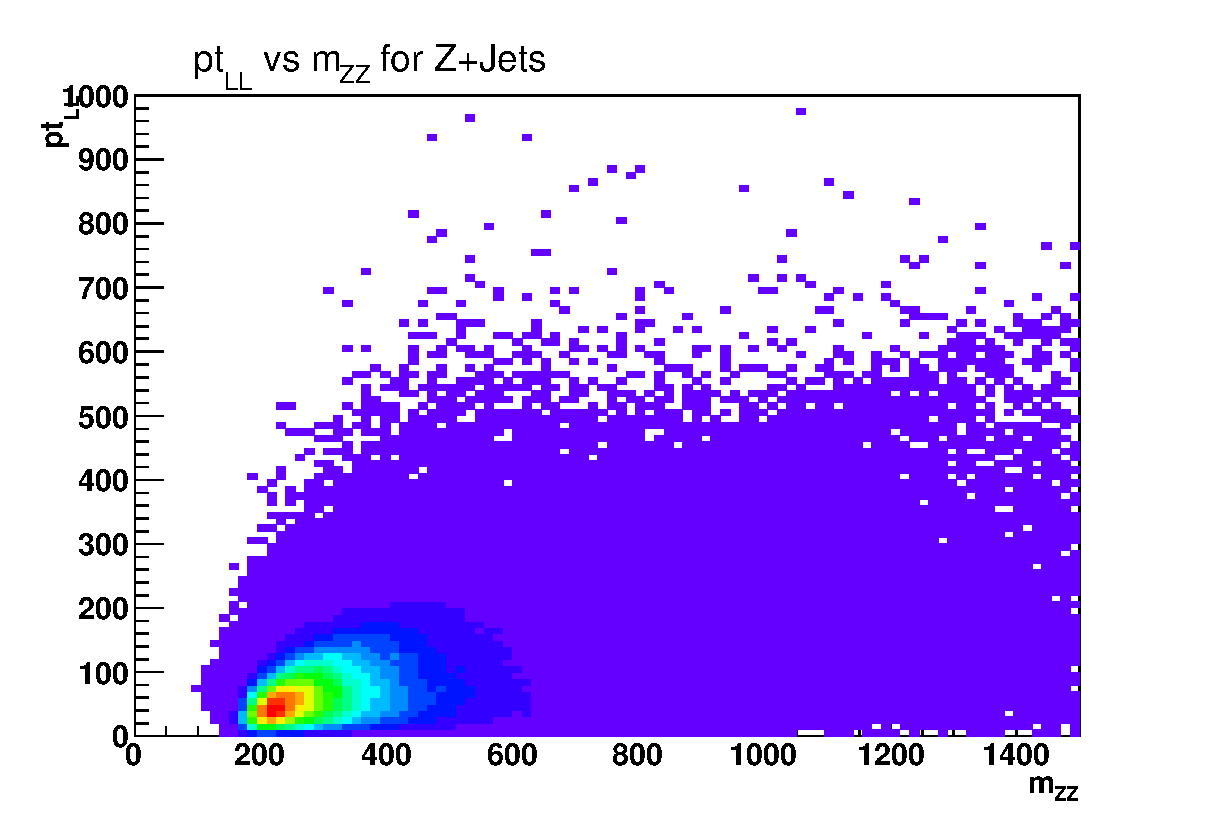
\includegraphics[width=0.45\textwidth]{Optimization/mzz_ptLL_background.eps}
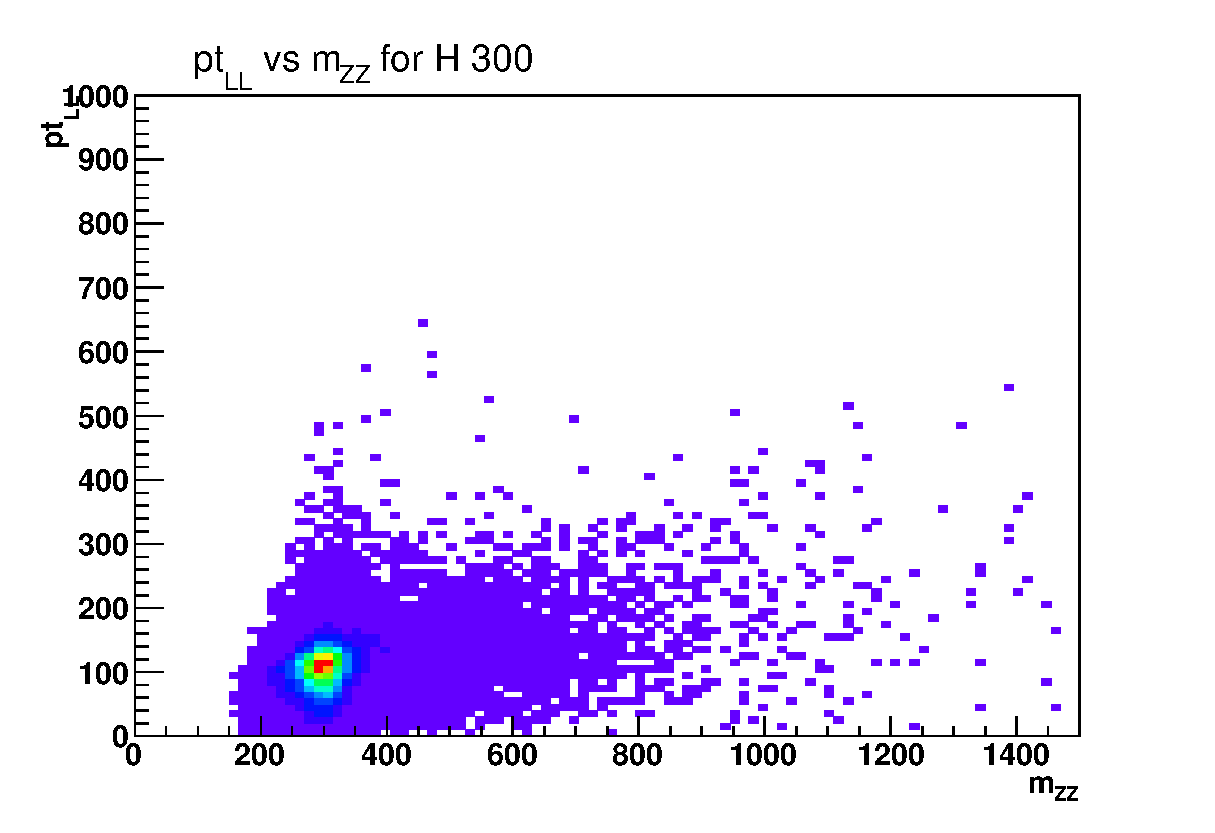
\includegraphics[width=0.45\textwidth]{Optimization/mzz_ptLL_300.eps}
}
\centerline{
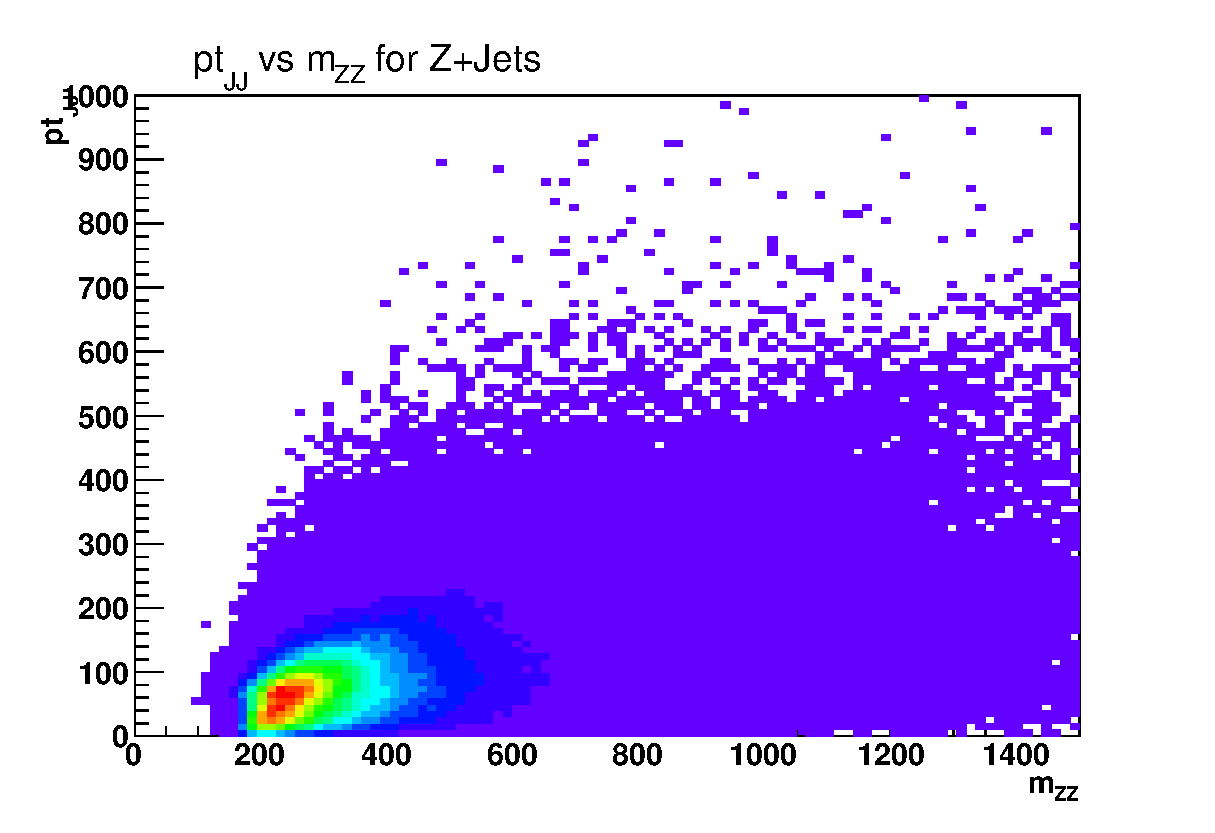
\includegraphics[width=0.45\textwidth]{Optimization/mzz_ptJJ_background.eps}
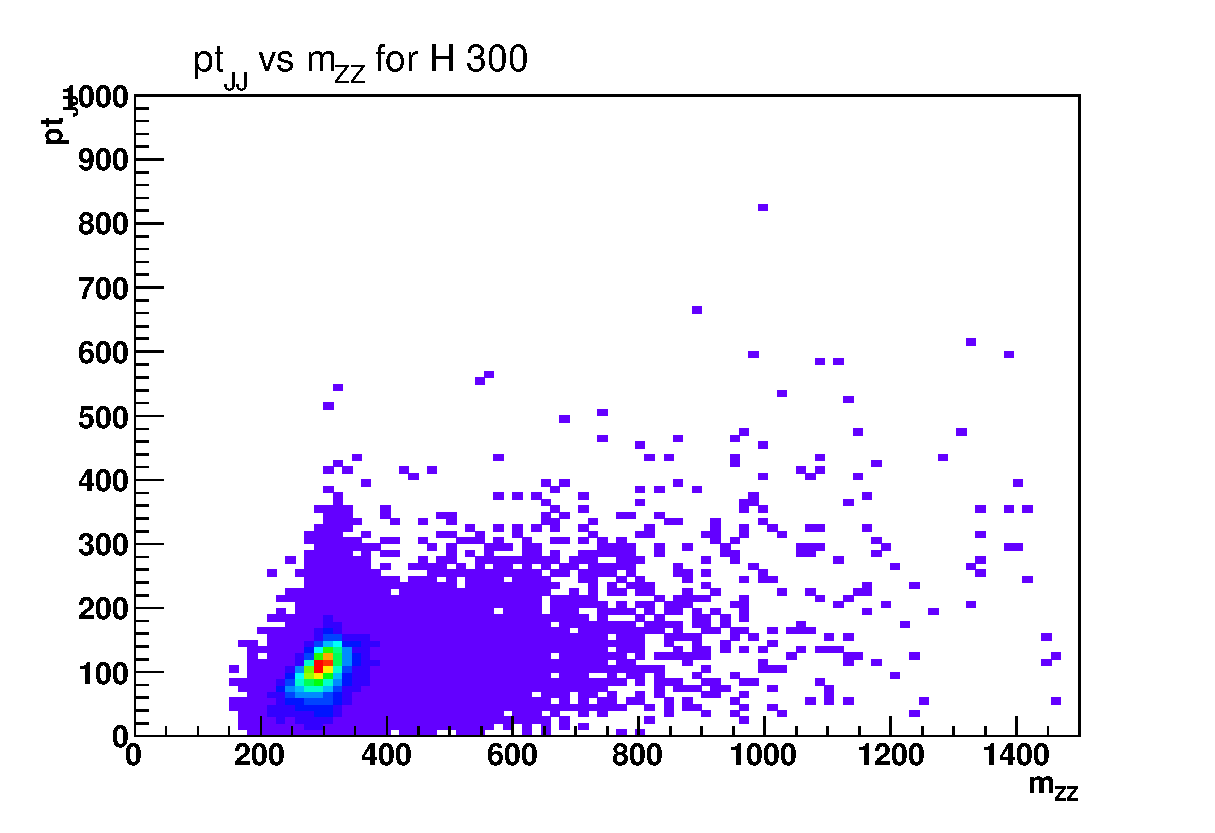
\includegraphics[width=0.45\textwidth]{Optimization/mzz_ptJJ_300.eps} \\
}
\centerline{
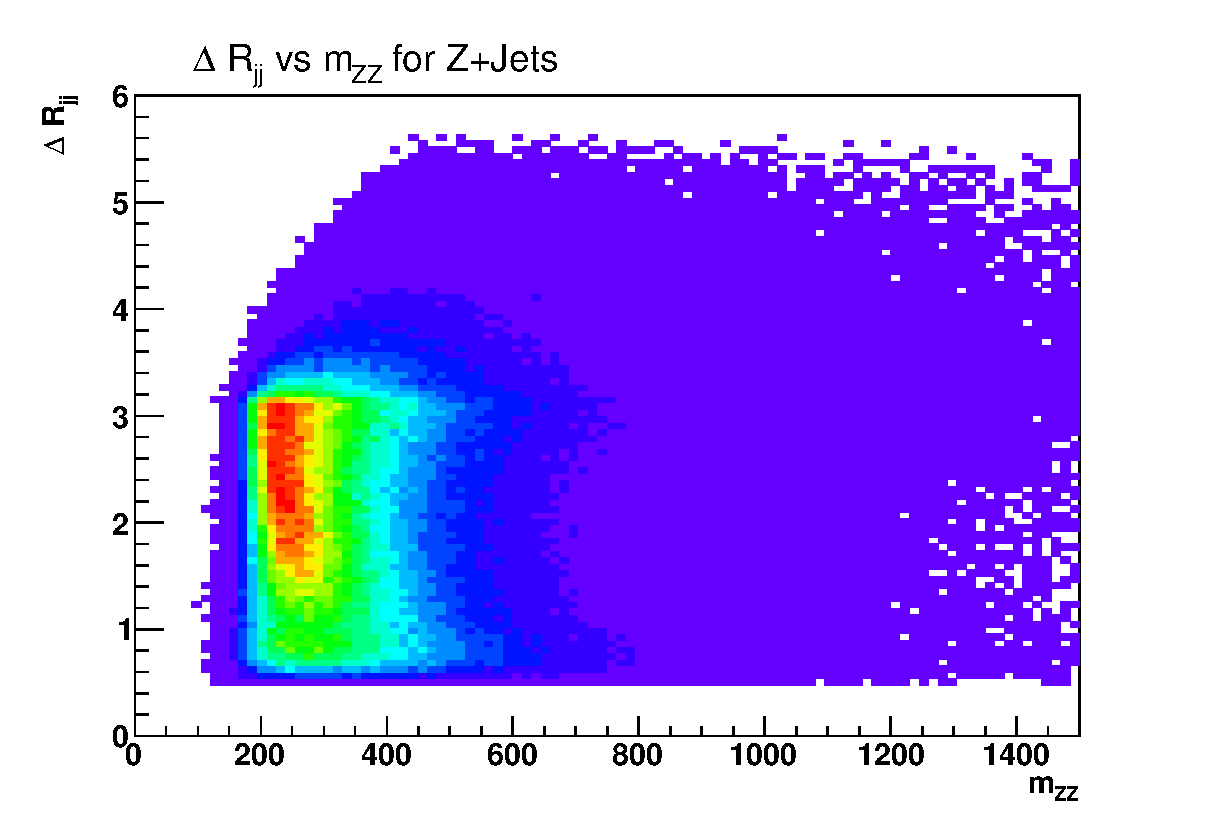
\includegraphics[width=0.45\textwidth]{Optimization/mzz_jjdr_background.eps}
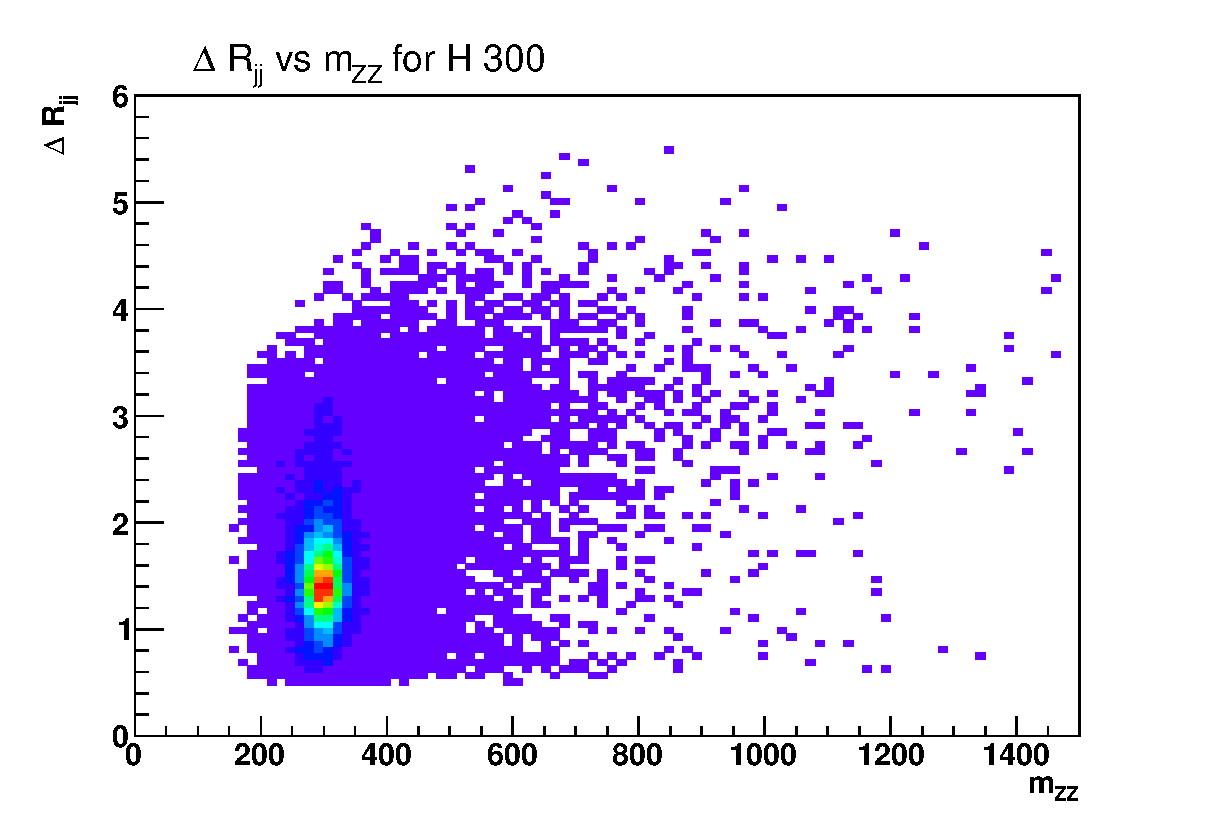
\includegraphics[width=0.45\textwidth]{Optimization/mzz_jjdr_300.eps} \\
%\includegraphics[height=2.5in]{plots/angles-Graviton-all2}
}
%\end{center}
\caption{Various kinematic variables comparing Z+Jets background and Higgs of 300 GeV simulations to demonstrate the correlation between the kinematics and $m_{ZZ}$.  (Top Left) $p_T (ll)$ vs $m_{ZZ}$ for Z+Jets.  (Top Right) $p_T (ll)$ vs $m_{ZZ}$ for Higgs 300. (Middle Left) $p_T (jj)$ vs $m_{ZZ}$ for Z+Jets.  (Middle Right) $p_T (jj)$ vs $m_{ZZ}$ for Higgs 300. (Bottom Left) $\Delta R_{jj}$ vs $m_{ZZ}$ for Z+Jets.  (Bottom Right) $\Delta R_{jj}$ vs $m_{ZZ}$ for Higgs 300. 
\label{fig:nousevars}}  
\end{figure}
%%%%%%%%%

The signal topology is affected by the production of a heavy Higgs.  These topological features are not limited to only the kinematics of the final state particles but have other manifestations as well.  This is because the decay of a spin-0 boson decays to a pair of identical spin-1 bosons which decay to fermions.  For us, the spin-0 boson is the Higgs and the spin-1 bosons are the Z bosons.  This well defined spin correlation will be seen in the angular distribution of the final state particles.  The probability density functions of the angles can be computed analytically for Higgs signals~\cite{Physics_2010}.  The background is not resonant so there is no spin correlation and thus there are different angular distributions for the final states between Z+Jets and the signal.  This topology difference is not unique to the Higgs boson and can also help in the search for other particles~\cite{PhysRevD.81.075022}. 

The decay kinematics in the signal $H \rightarrow ZZ \rightarrow 2l2q$ have several distinct features that can be used to discriminate against background. Five angular observables fully describe the angular distribution of the decay products in $2 \rightarrow 1 \rightarrow 2 \rightarrow 4$ as in $ab \rightarrow X \rightarrow ZZ \rightarrow 2l2j$ ~\cite{Gao_5angles,Rujela_5angles}. There are three helicity angles $\theta_1, \theta_2,$ and $\Phi$, as well as two production angels $\theta^*$ and $\Phi_1$.  Additionally, they are orthogonal to the three invariant masses of the $X$ and the two $Z$ and to the longitudinal and transverse momenta of the $X$. The orthogonal observables are largely uncorrelated and are useful for event selection beyond using them as raw kinematic observables. The definitions of these variables can be found in Table~\ref{tab:5anglesdef}.
Fig.~\ref{fig:decay} illustrates the angular distribution in the production and decay chain $ab\to X\to P_1P_2\to p_{11}p_{12}p_{21}p_{22}$ with an example of the $ab\to X\to ZZ\to 2\ell2q$ chain with two partons $a$ and $b$, such as $gg$ or $q\bar{q}$.

%%%%%%%%%%%%%%%%%%%%%%%%%%%%%%%%
\begin{table*}[htb!]
\caption{ 
Definitions of the 5 angular variables describing events of the form $ab \rightarrow X \rightarrow ZZ \rightarrow 2l2j$ as seen in Figure~\ref{fig:decay}.
}
\label{tab:5anglesdef}
\vspace*{\medskipamount}
\begin{center}
\small
\begin{tabularx}{\textwidth}{|c|X|}
%\begin{tabular}{|c|l|}
\hline
Variable & Definition\\
\hline
$\theta_1$ & The angle between the direction of the $\Plm$ (from $Z \rightarrow \Plp \Plm$) and the direction opposite the X in the Z rest frame. \\ \hline
$\theta_2$ & The angle between the direction of the $\Pq$ (from $Z \rightarrow \Pq \Paq$) and the direction opposite the X in the Z rest frame. \\ \hline
$\Phi$ & The angle between the decay planes of the two Z decays. \\ \hline
$\theta^*$ & The angle between the parton collision axis ($z$) and the decay axis in the rest frame ($z^`$). \\ \hline
$\Phi_1$ & The angle between the production plane and the $Z \rightarrow \Plp \Plm$ decay plane. \\
\hline
\end{tabularx}
\end{center}
\end{table*}
%%%%%%%%%%%%%%%%%%%%%%%%%%%%%%%%%%%%%%%%%%%%%%%%%


%%%%%%%%%
\begin{figure}[htb!]
%\begin{center}
\centerline{
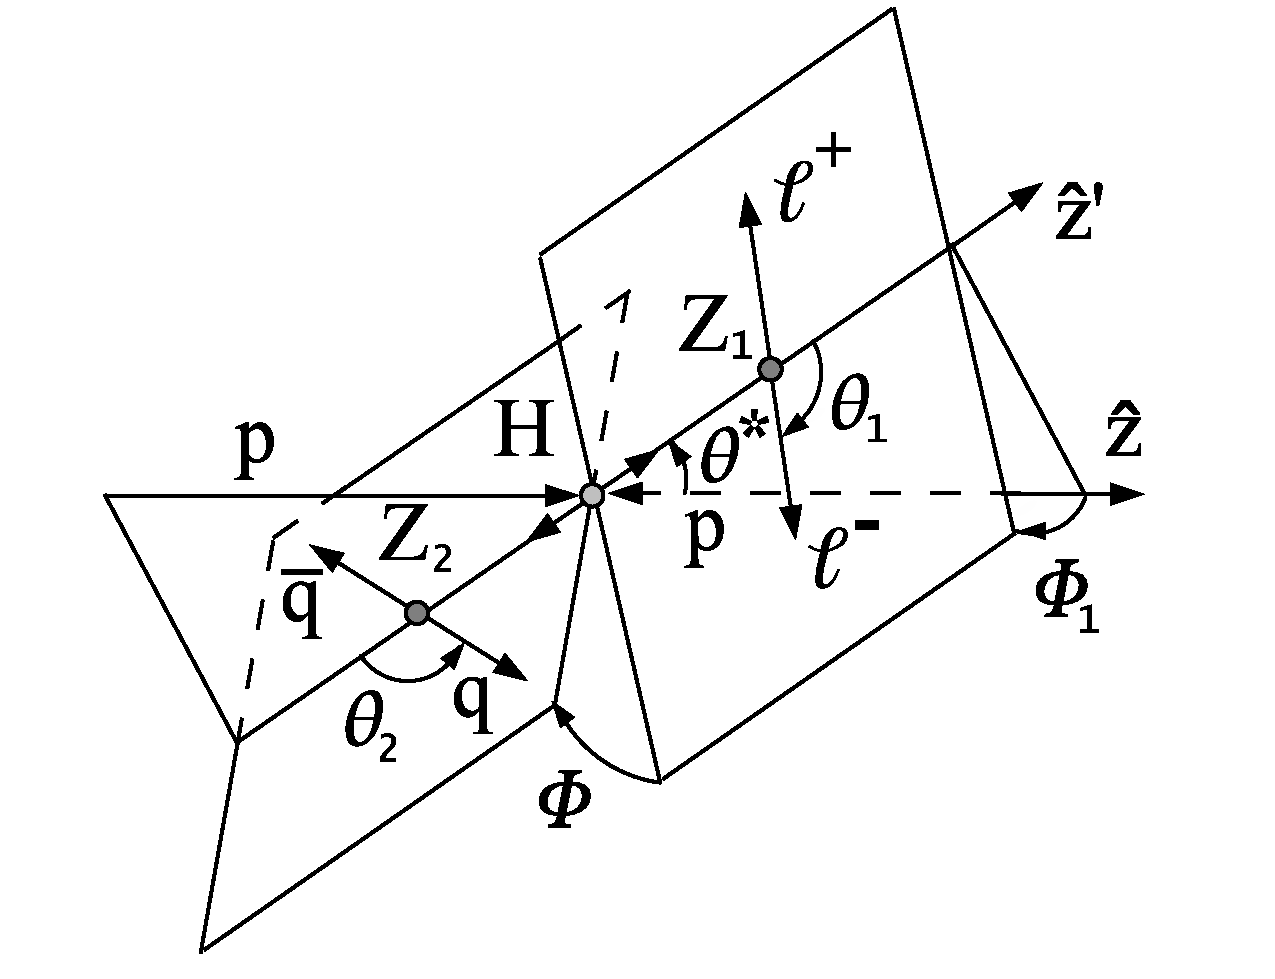
\includegraphics[height=2.5in]{plots/angles-HZZ2l2q}
%\includegraphics[height=2.5in]{plots/angles-Graviton-all2}
}
%\end{center}
\caption{Diagram depicting the decay $X\rightarrow ZZ\rightarrow 2l2q$ and the 5 decay angles which describe it.
\label{fig:decay}}
\end{figure}
%%%%%%%%%


The angular distributions for data and simulations can be found in Figures~\ref{helicityDistDataMCE0},~\ref{helicityDistDataMCE1}, and~\ref{helicityDistDataMCE2} for electrons and in Figures~\ref{helicityDistDataMCM0},~\ref{helicityDistDataMCM1}, and~\ref{helicityDistDataMCM2} for muons.  These figures show the differences between the samples in each of the b-tag regions.  Because the background does not have spin correlation, there is a difference between the simulated signal, the background simulation, and data.  Also, you can see similar performance between electrons and muons, as well as between different b-tag categories.  This similarity between muons and electrons, as well as between b-tag categories, is expected and will be used to simplify the analysis by doing common final selection between lepton types and b-tag categories.


%%%%%%%%%%%%%
\begin{figure}[thb!]
\centerline{
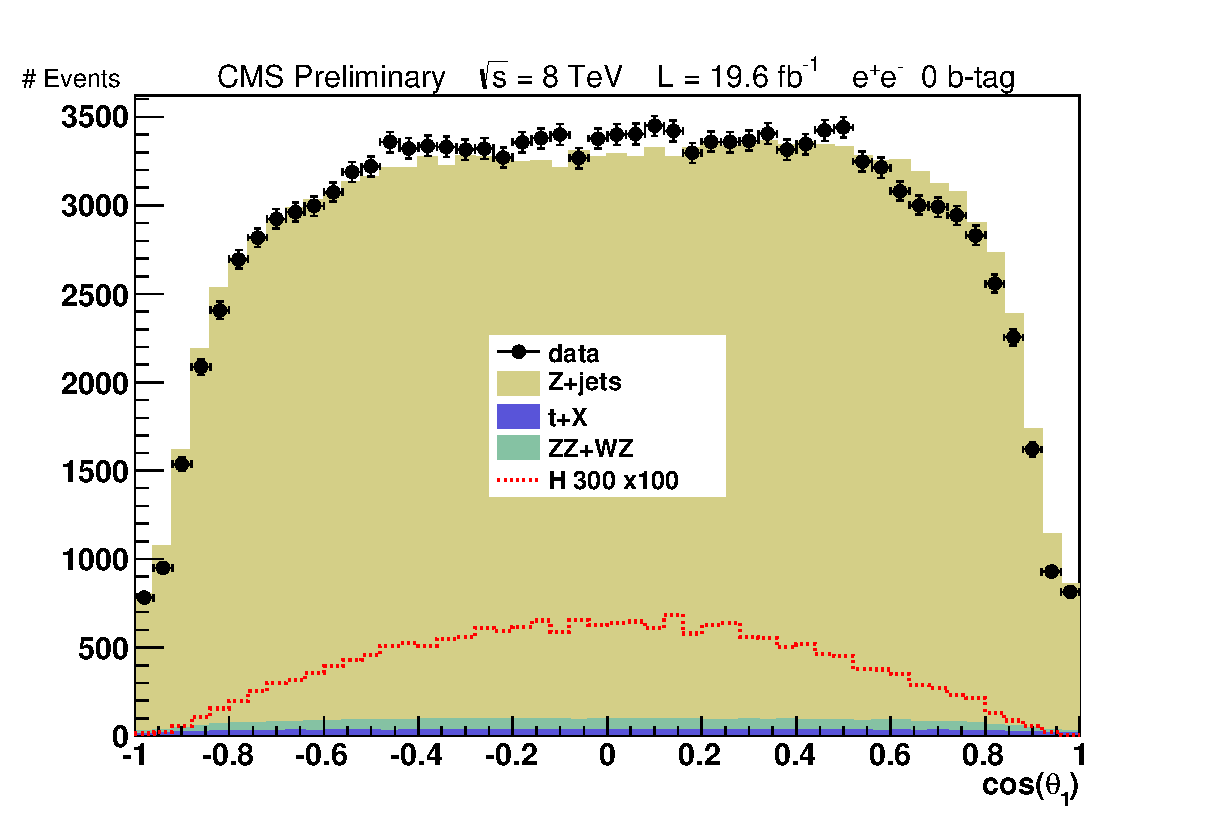
\includegraphics[width=0.33\textwidth]{presentation/defense/images/preselection/0/el/costheta1.eps}
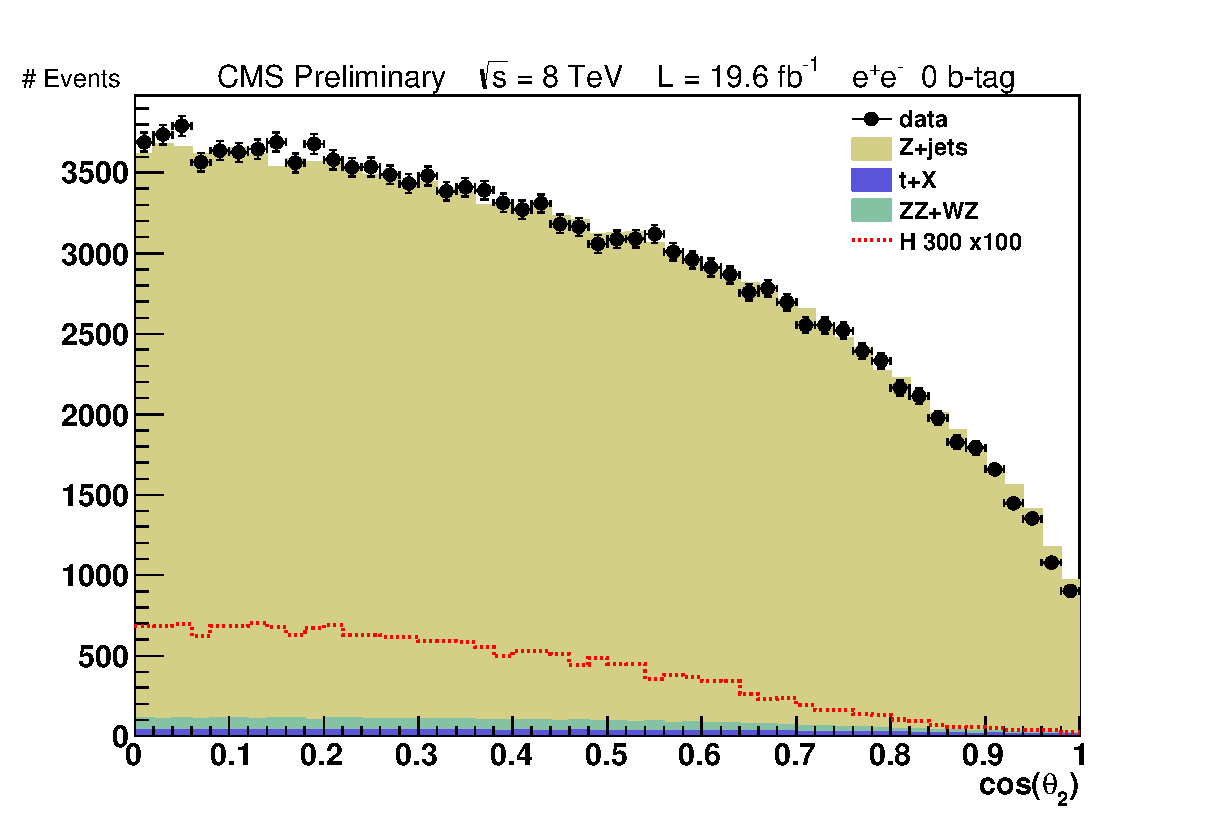
\includegraphics[width=0.33\textwidth]{presentation/defense/images/preselection/0/el/costheta2.eps}
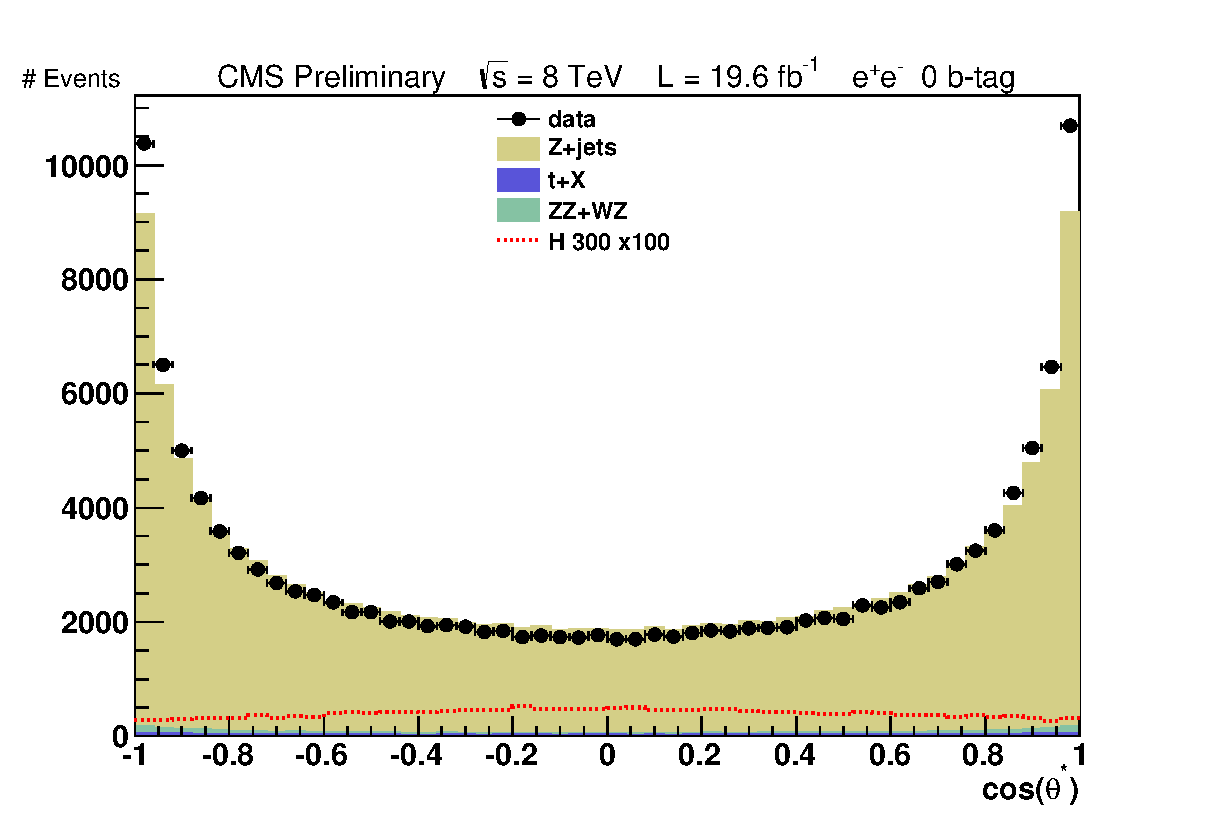
\includegraphics[width=0.33\textwidth]{presentation/defense/images/preselection/0/el/costhetast.eps}
}
\centerline{
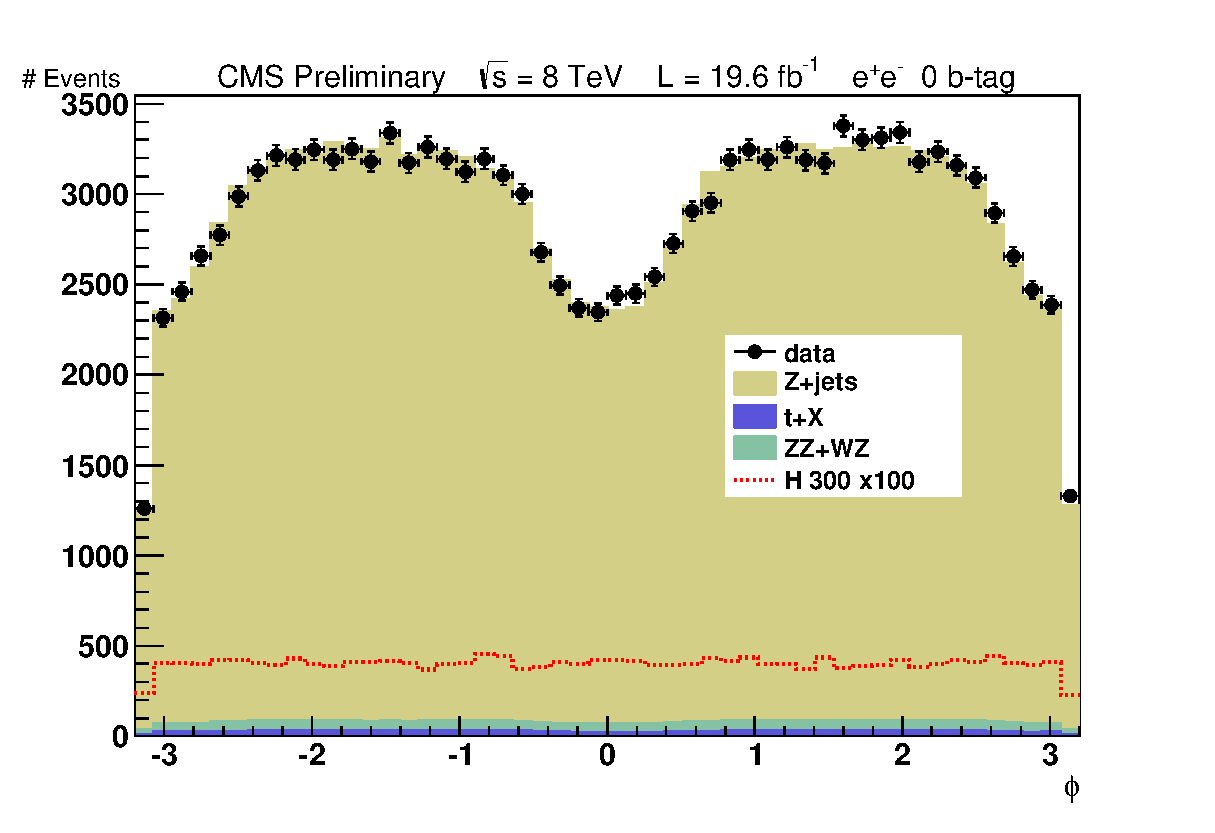
\includegraphics[width=0.33\textwidth]{presentation/defense/images/preselection/0/el/phi.eps}
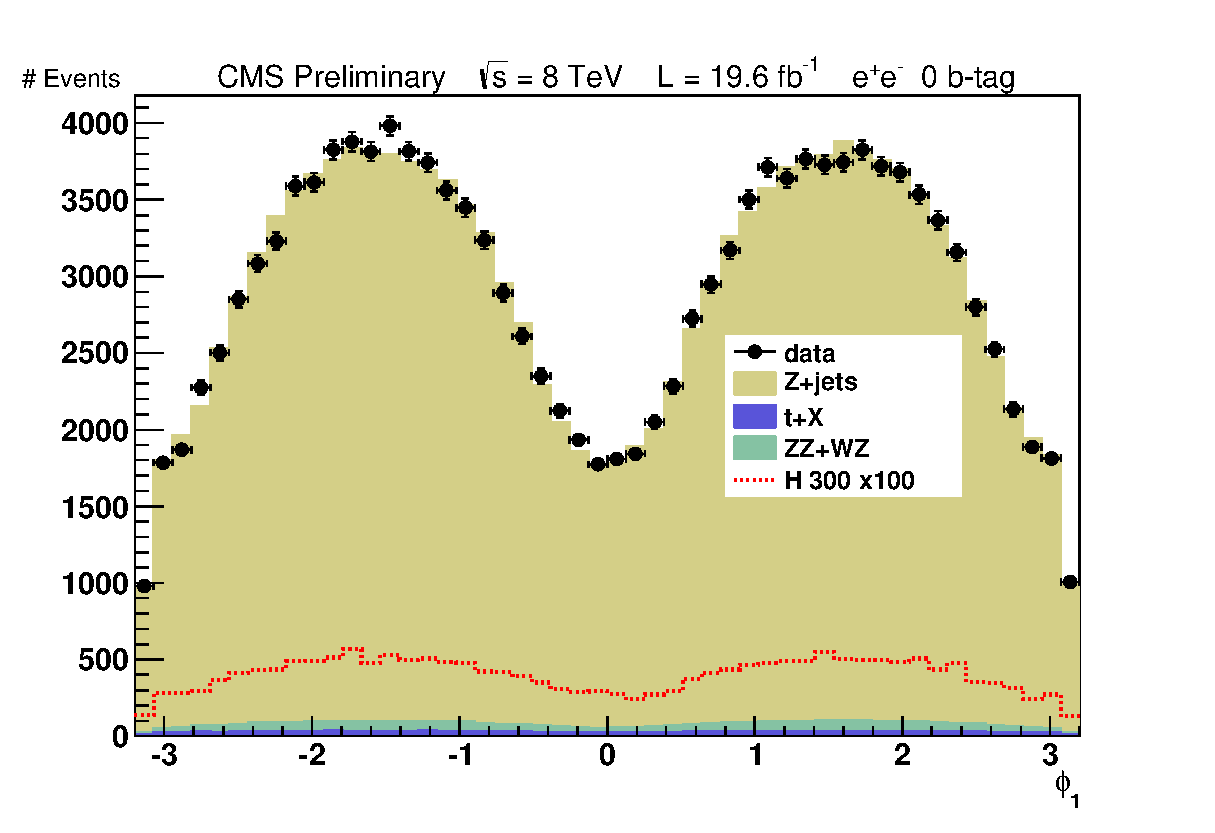
\includegraphics[width=0.33\textwidth]{presentation/defense/images/preselection/0/el/phi1.eps}
}
\caption{
Five angular distributions of $\cos\theta_1, \cos\theta_2, \cos\theta^*, \Phi$, $\Phi_1$ and the helicity likelihood discriminant for 2012 electron data (points) and Summer 2012 Monte Carlo samples (histogram) in the 0 b-tag category.  The red line is the expected distribution for a Higgs boson with mass 300 GeV.  The selection is as described in preselection.
\label{helicityDistDataMCE0}}
\end{figure}
%%%%%%%%%%%%%
%%%%%%%%%%%%%
\begin{figure}[thb!]
\centerline{
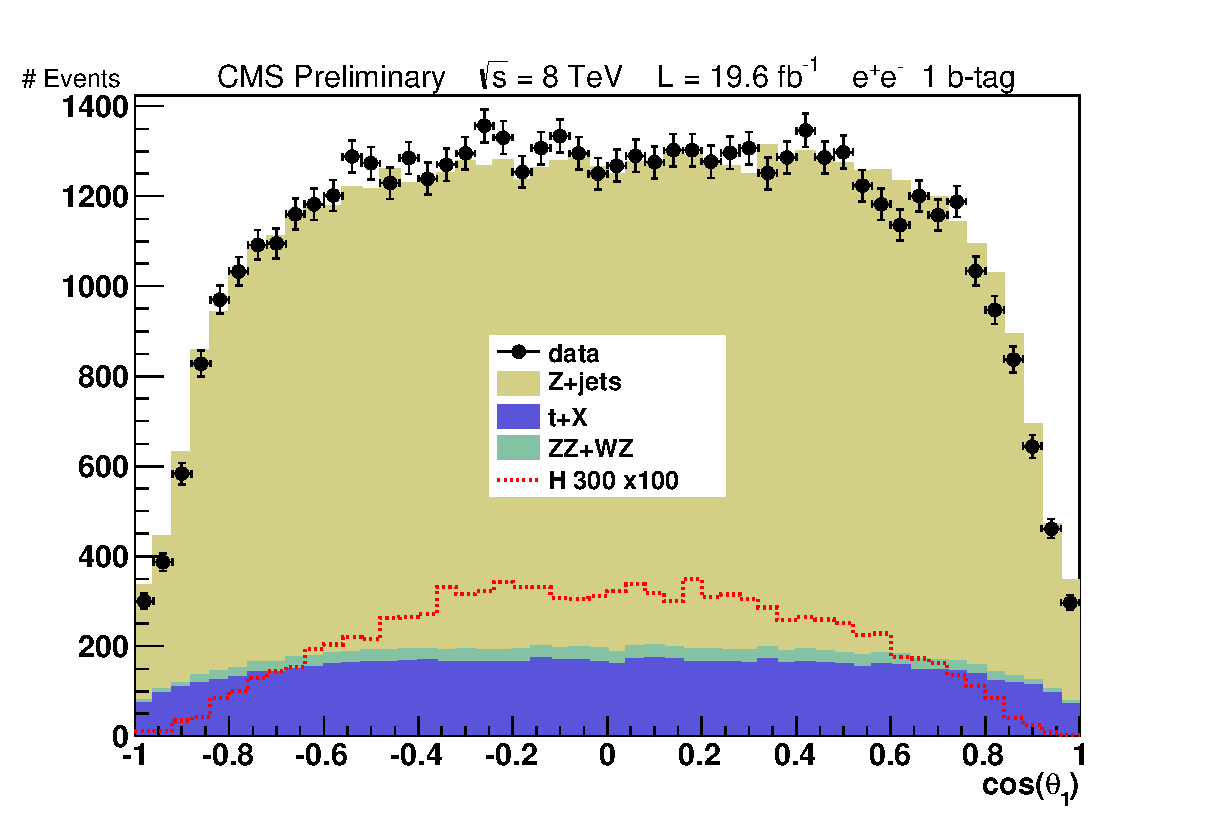
\includegraphics[width=0.33\textwidth]{presentation/defense/images/preselection/1/el/costheta1.eps}
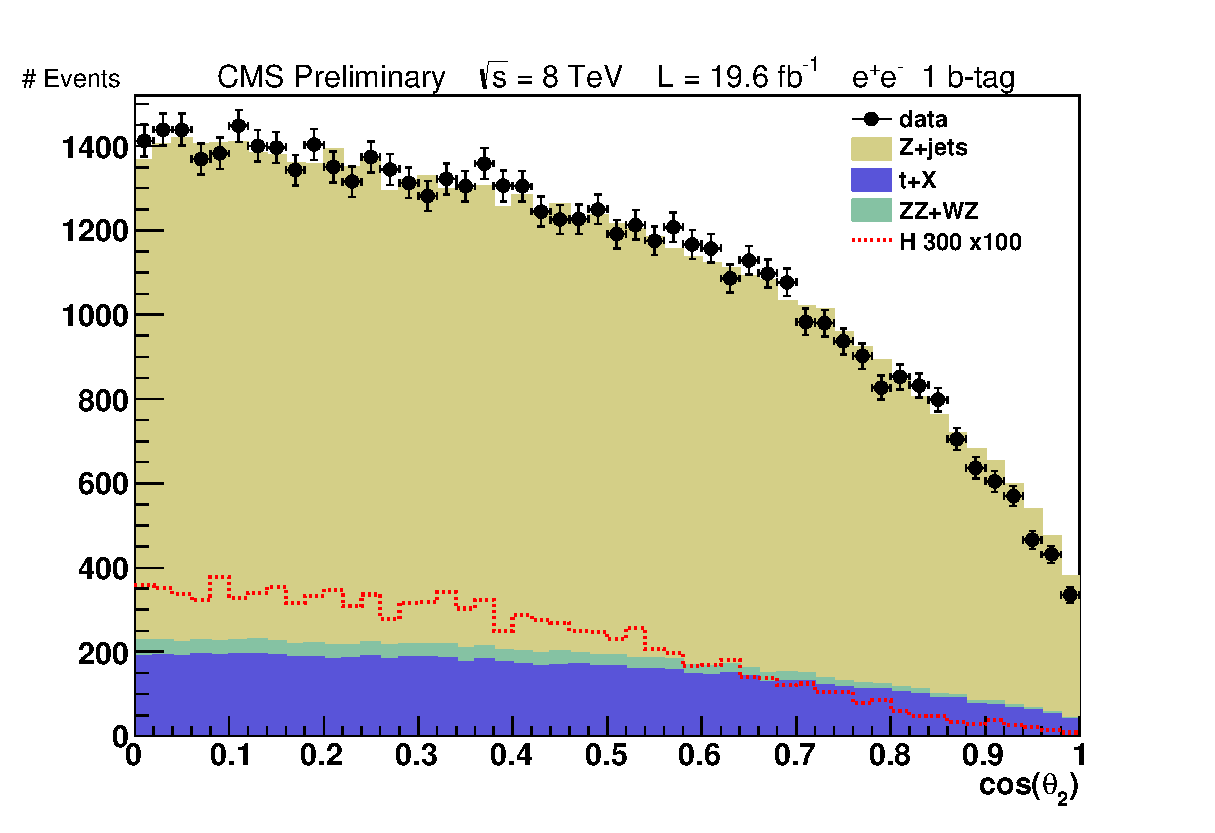
\includegraphics[width=0.33\textwidth]{presentation/defense/images/preselection/1/el/costheta2.eps}
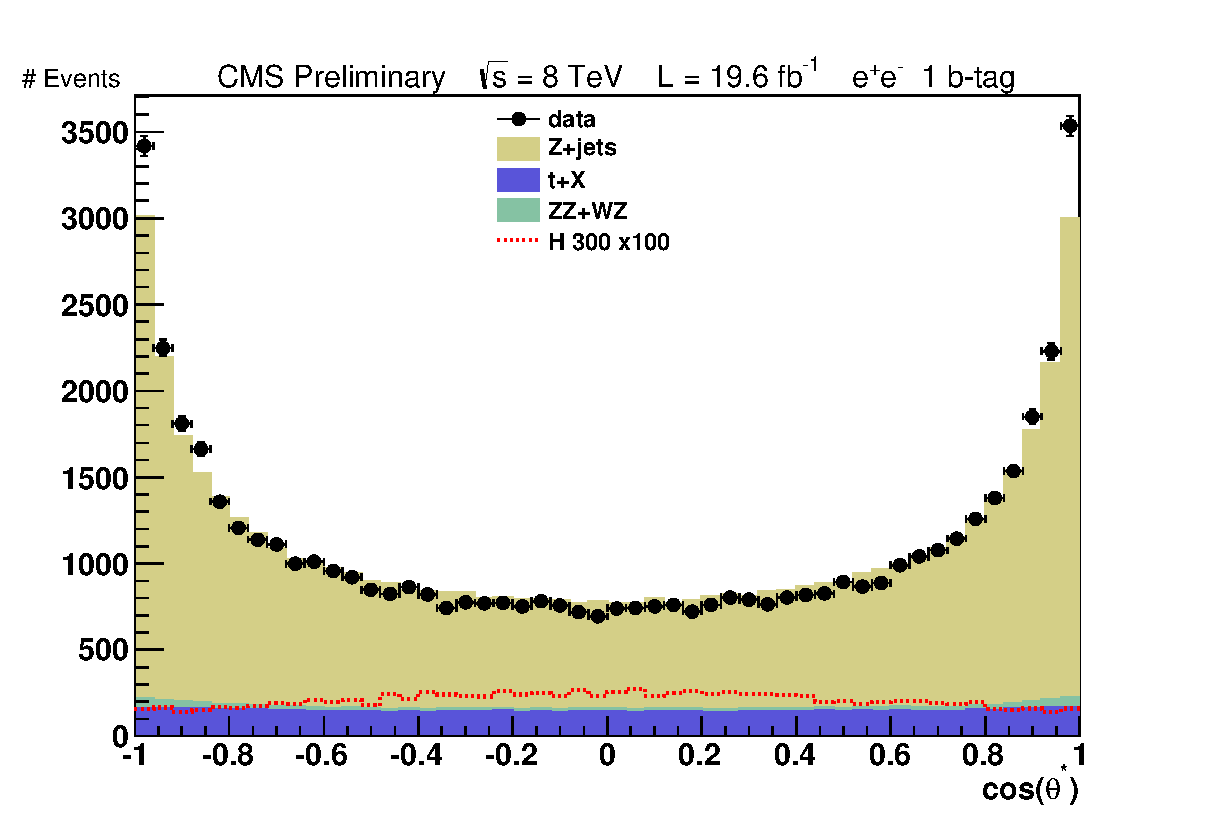
\includegraphics[width=0.33\textwidth]{presentation/defense/images/preselection/1/el/costhetast.eps}
}
\centerline{
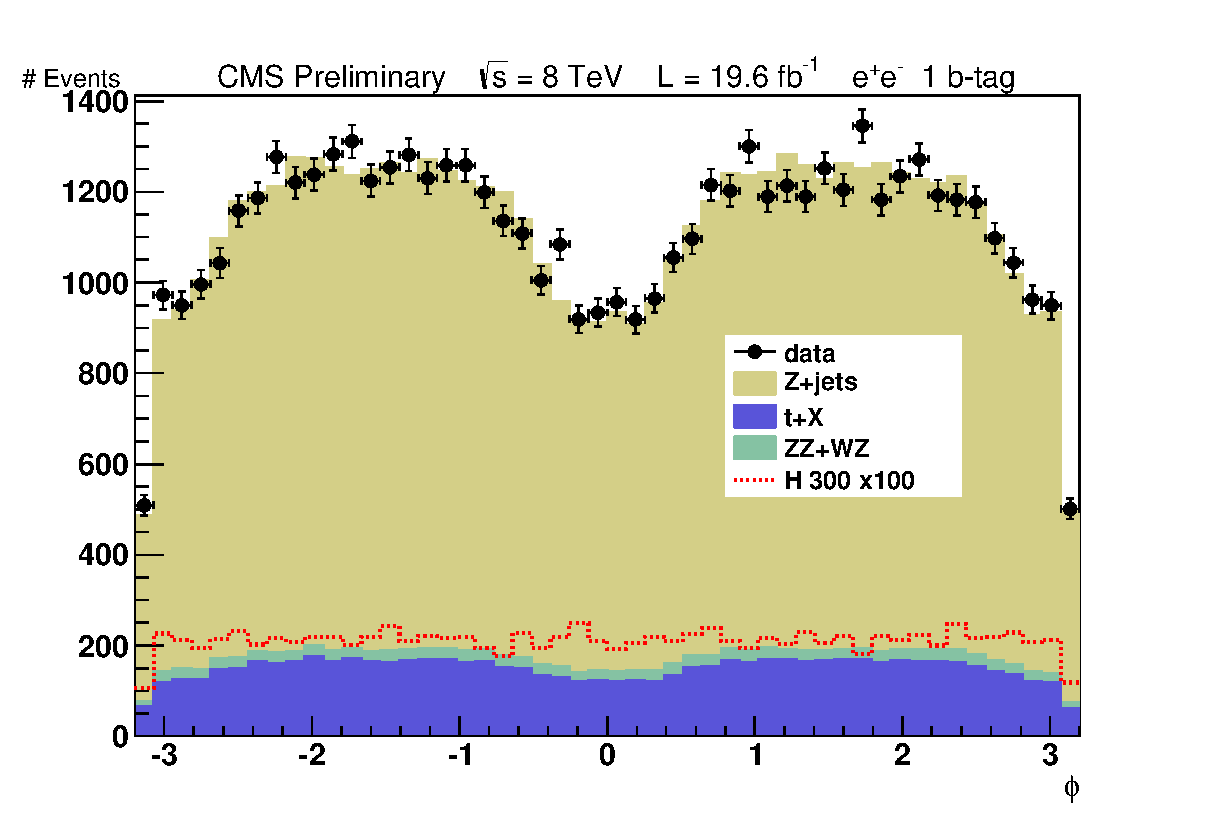
\includegraphics[width=0.33\textwidth]{presentation/defense/images/preselection/1/el/phi.eps}
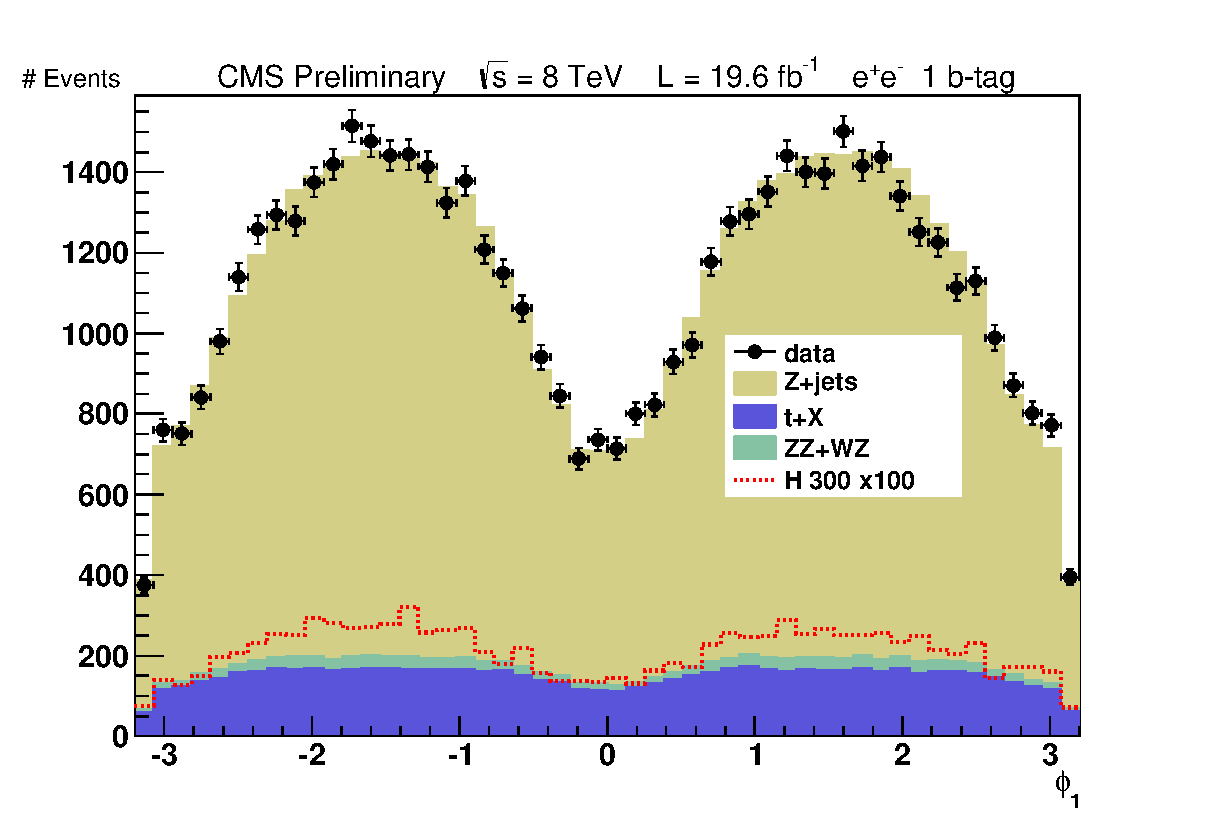
\includegraphics[width=0.33\textwidth]{presentation/defense/images/preselection/1/el/phi1.eps}
}
\caption{
Five angular distributions of $\cos\theta_1, \cos\theta_2, \cos\theta^*, \Phi$, $\Phi_1$ and the helicity likelihood discriminant for 2012 electron data (points) and Summer 12 Monte Carlo samples (histogram) in the 1 b-tag category.  Open histograms indicate the expected distribution for a Higgs boson with mass 300 GeV. The selection is as described in preselection.
\label{helicityDistDataMCE1}}
\end{figure}
%%%%%%%%%%%%%
%%%%%%%%%%%%%
\begin{figure}[thb!]
\centerline{
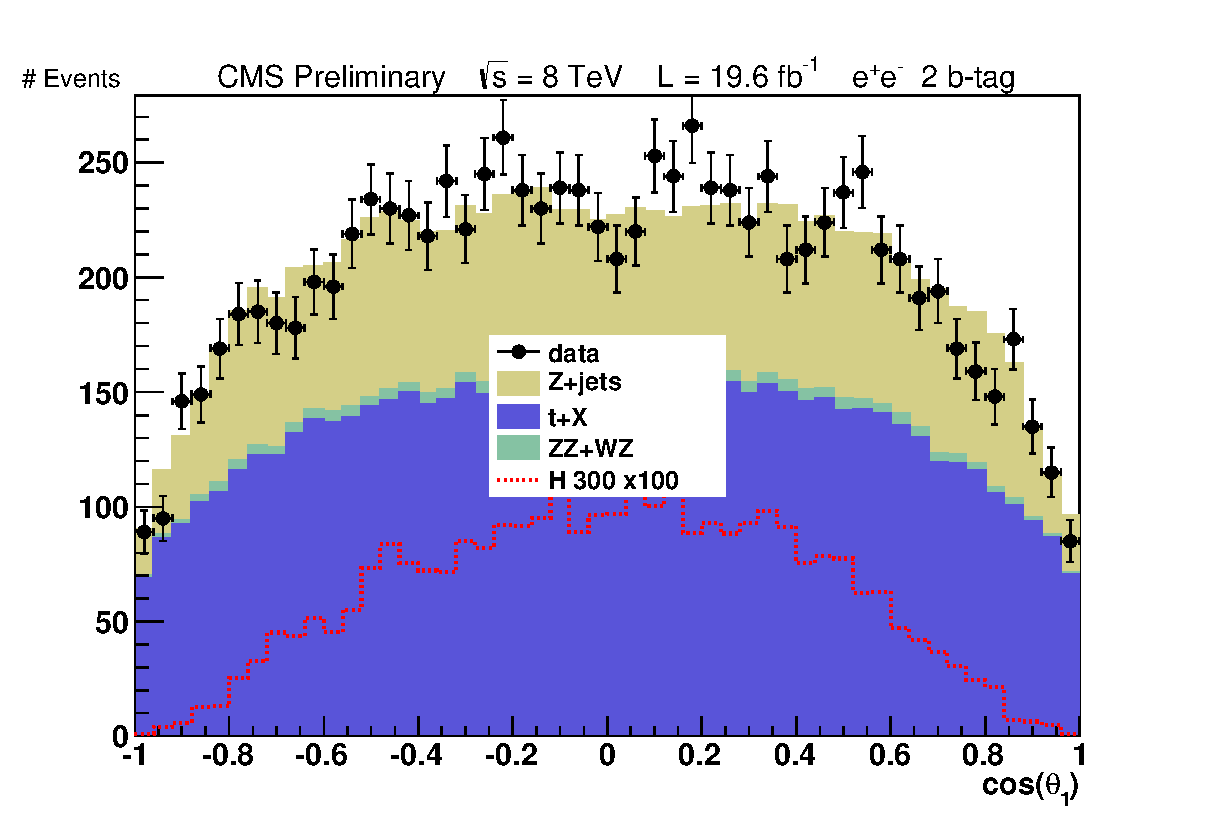
\includegraphics[width=0.33\textwidth]{presentation/defense/images/preselection/2/el/costheta1.eps}
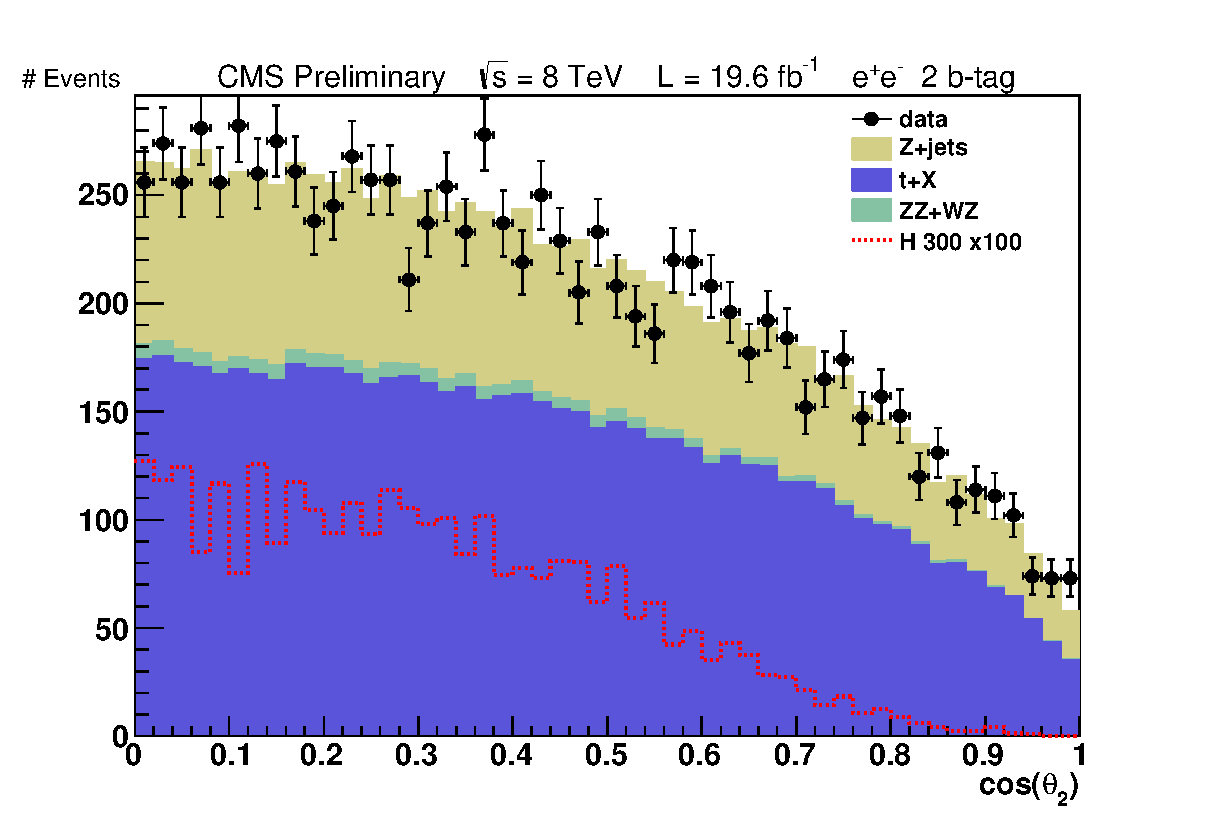
\includegraphics[width=0.33\textwidth]{presentation/defense/images/preselection/2/el/costheta2.eps}
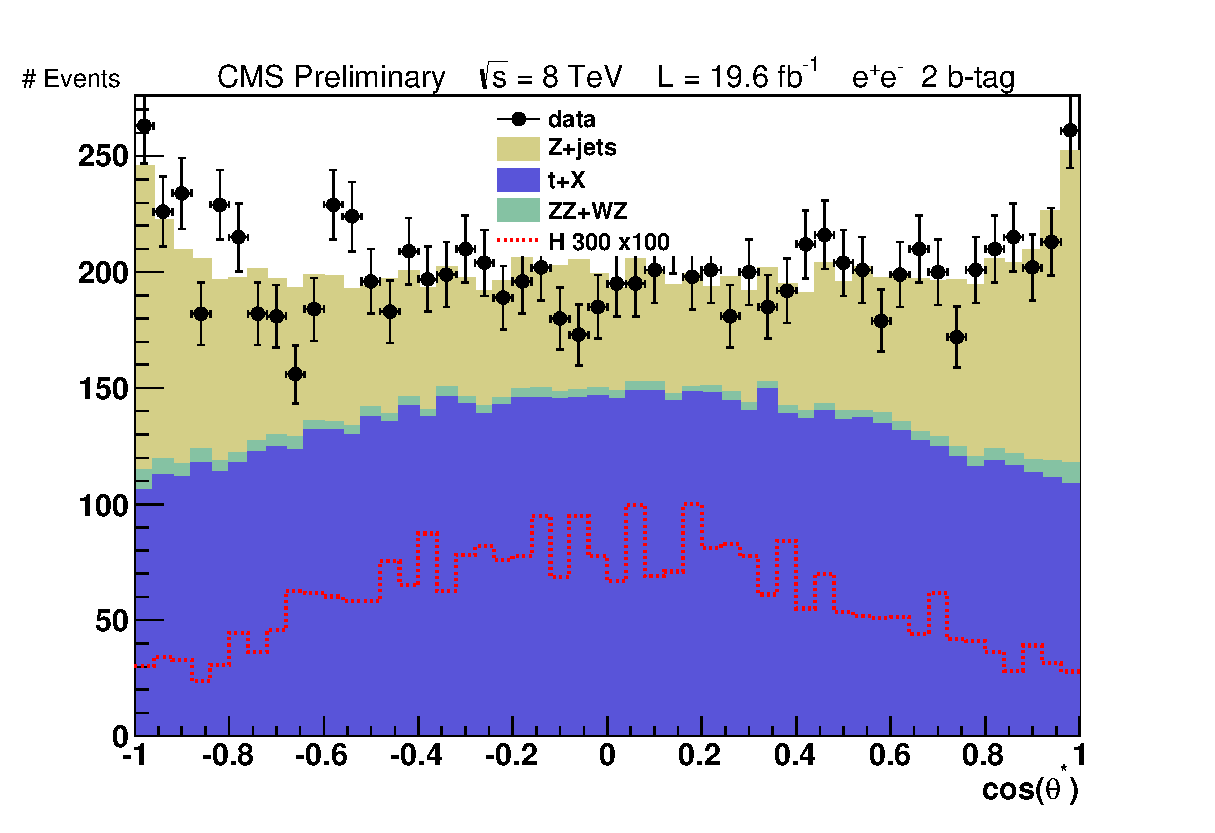
\includegraphics[width=0.33\textwidth]{presentation/defense/images/preselection/2/el/costhetast.eps}
}
\centerline{
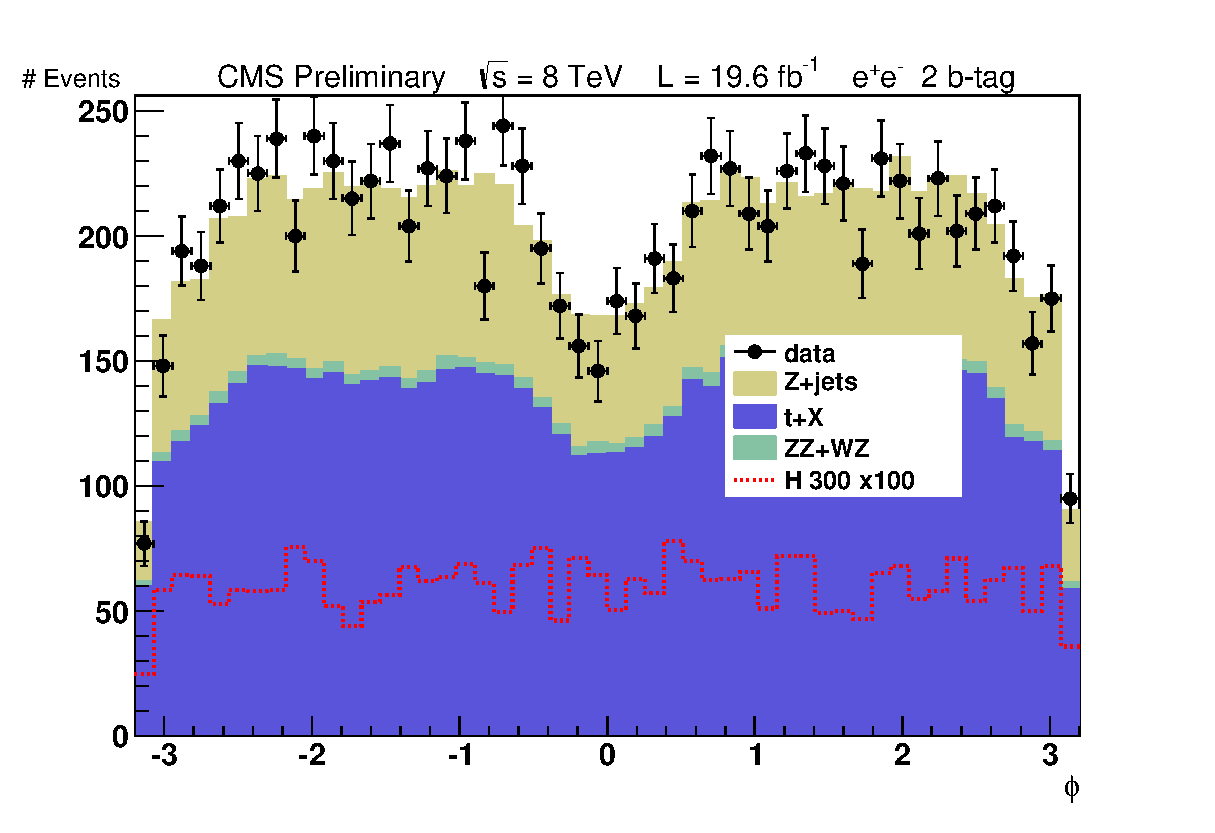
\includegraphics[width=0.33\textwidth]{presentation/defense/images/preselection/2/el/phi.eps}
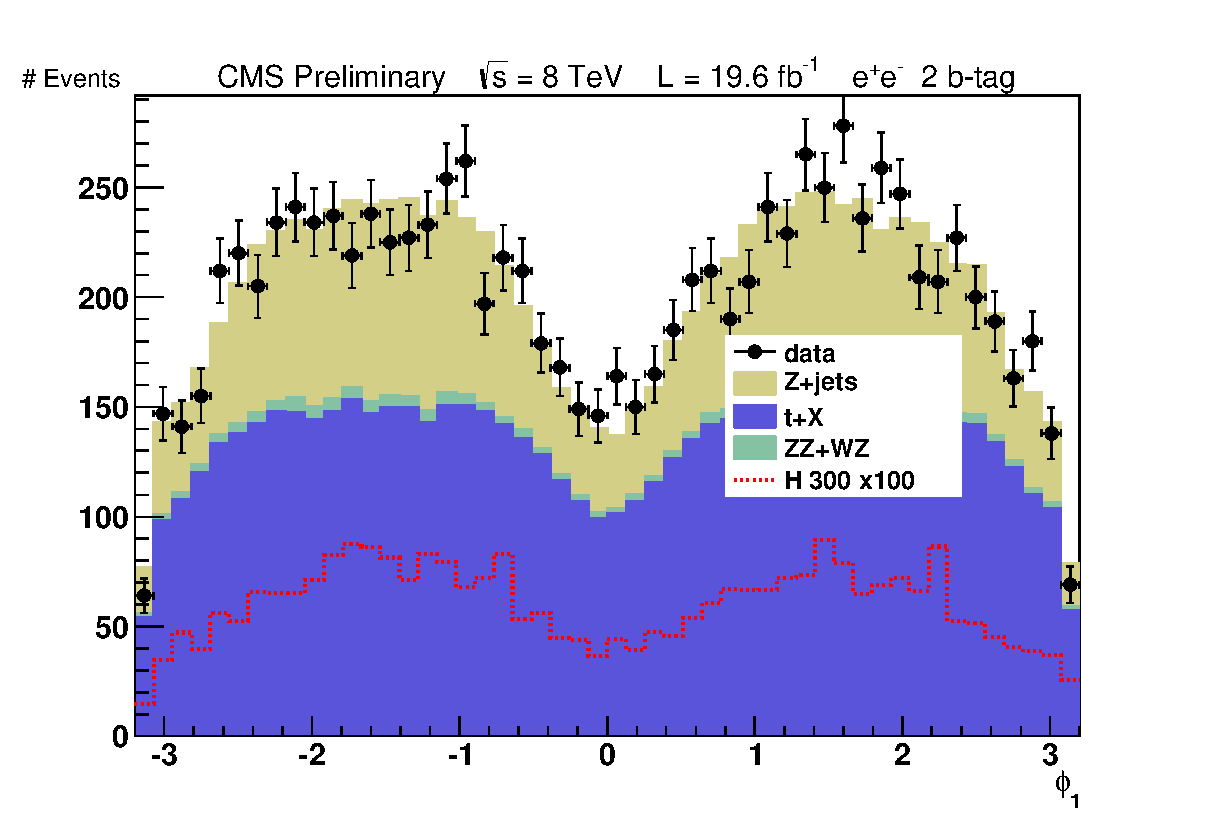
\includegraphics[width=0.33\textwidth]{presentation/defense/images/preselection/2/el/phi1.eps}
}
\caption{
Five angular distributions of $\cos\theta_1, \cos\theta_2, \cos\theta^*, \Phi$, $\Phi_1$ and the helicity likelihood discriminant for 2012 electron data (points) and Summer 12 Monte Carlo samples (histogram) in the 2 b-tag category.  Open histograms indicate the expected distribution for a Higgs boson with mass 300 GeV. The selection is as described in preselection.
\label{helicityDistDataMCE2}}
\end{figure}
%%%%%%%%%%%%%
%**********Muons******************%
%%%%%%%%%%%%%
\begin{figure}[thb!]
\centerline{
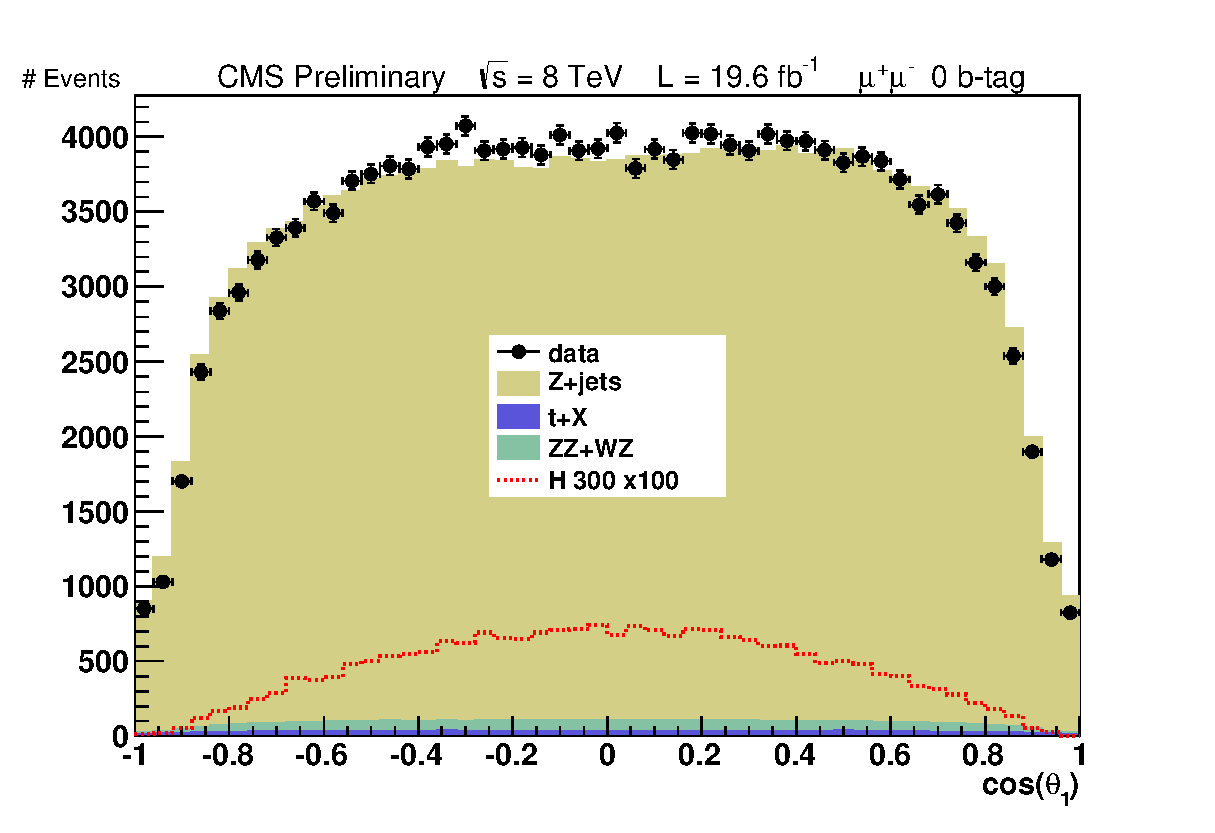
\includegraphics[width=0.33\textwidth]{presentation/defense/images/preselection/0/mu/costheta1.eps}
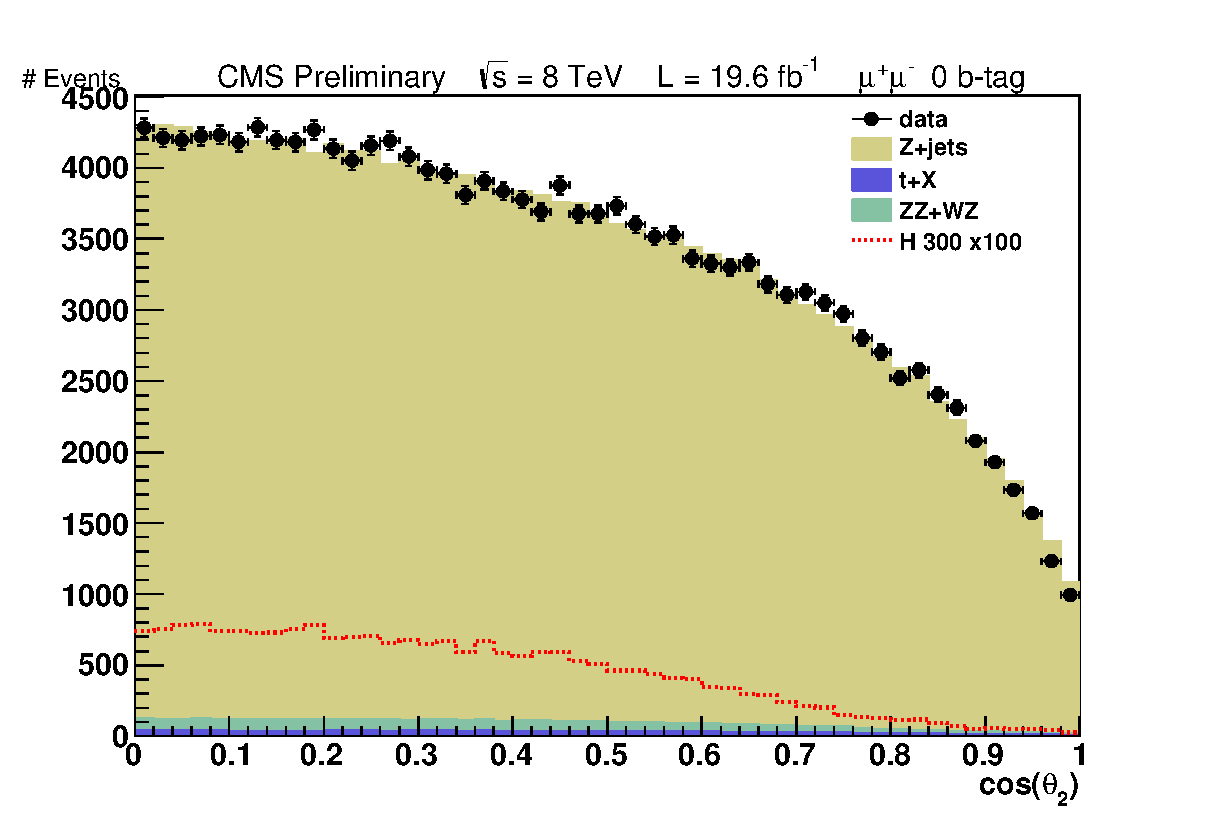
\includegraphics[width=0.33\textwidth]{presentation/defense/images/preselection/0/mu/costheta2.eps}
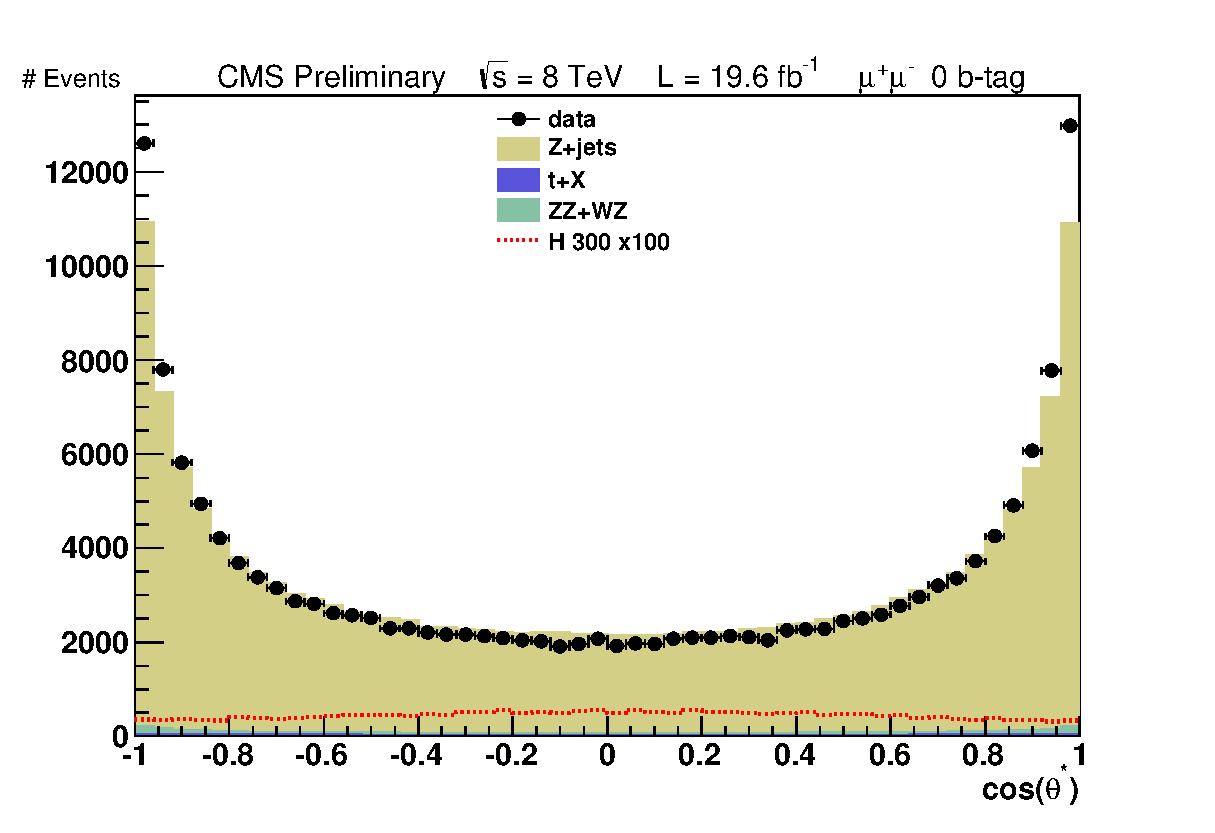
\includegraphics[width=0.33\textwidth]{presentation/defense/images/preselection/0/mu/costhetast.eps}
}
\centerline{
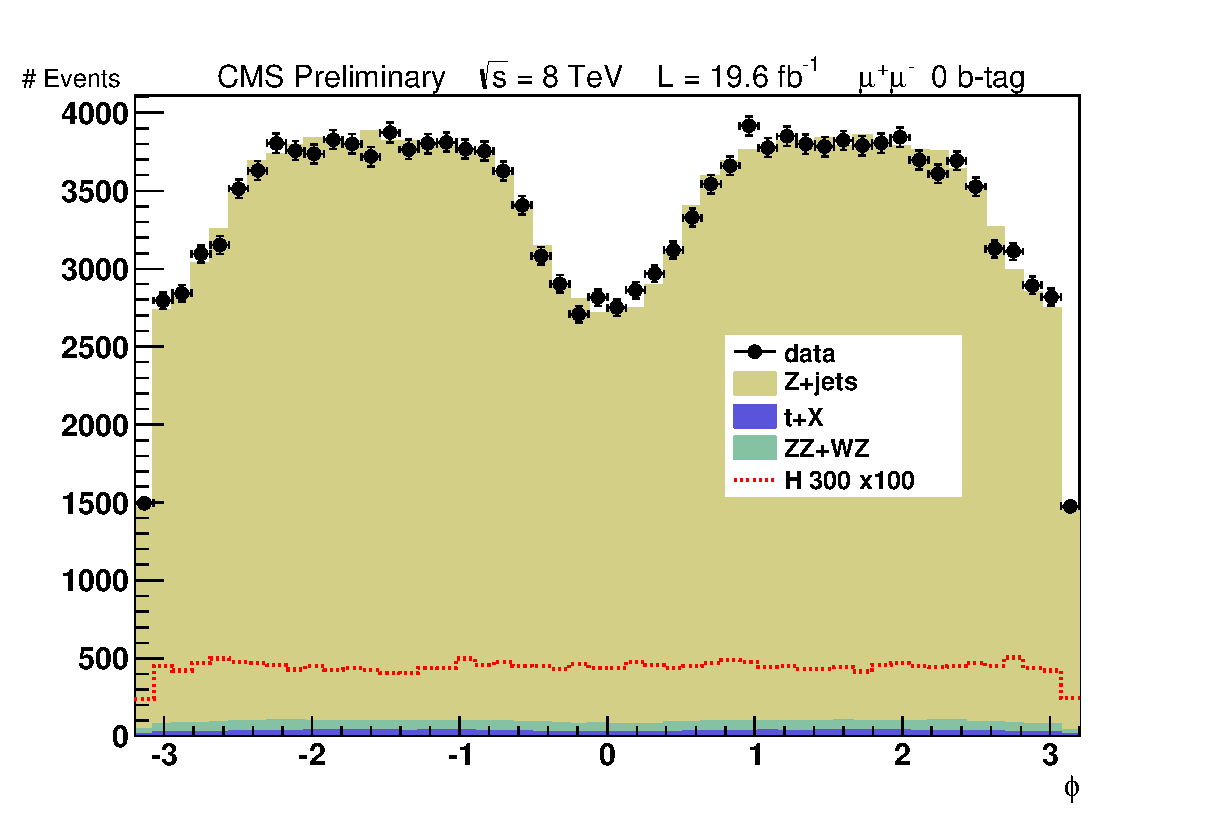
\includegraphics[width=0.33\textwidth]{presentation/defense/images/preselection/0/mu/phi.eps}
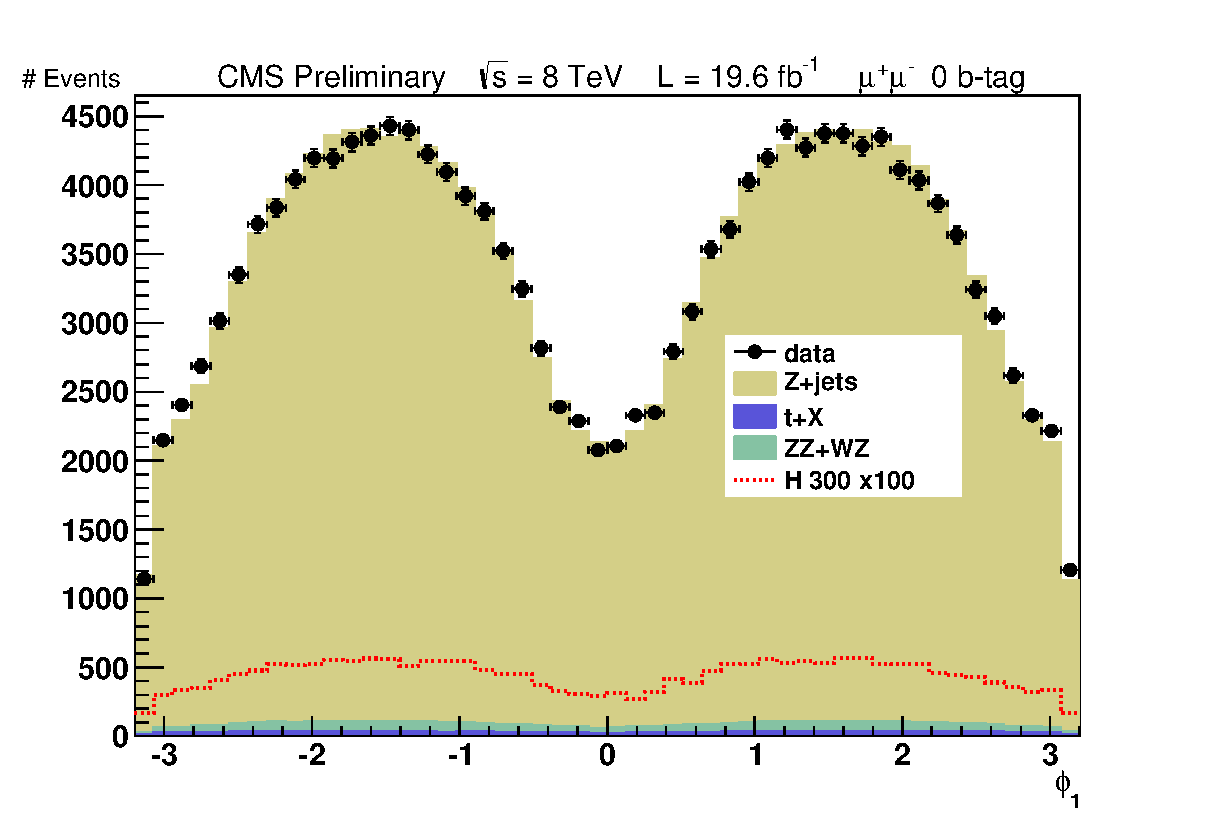
\includegraphics[width=0.33\textwidth]{presentation/defense/images/preselection/0/mu/phi1.eps}
}
\caption{
Five angular distributions of $\cos\theta_1, \cos\theta_2, \cos\theta^*, \Phi$, $\Phi_1$ and the helicity likelihood discriminant for 2012 muon data (points) and Summer 12 Monte Carlo samples (histogram) in the 0 b-tag category.  The red line is the expected distribution for a Higgs boson with mass 300 GeV.  The selection is as described in preselection.
\label{helicityDistDataMCM0}}
\end{figure}
%%%%%%%%%%%%%
%%%%%%%%%%%%%
\begin{figure}[thb!]
\centerline{
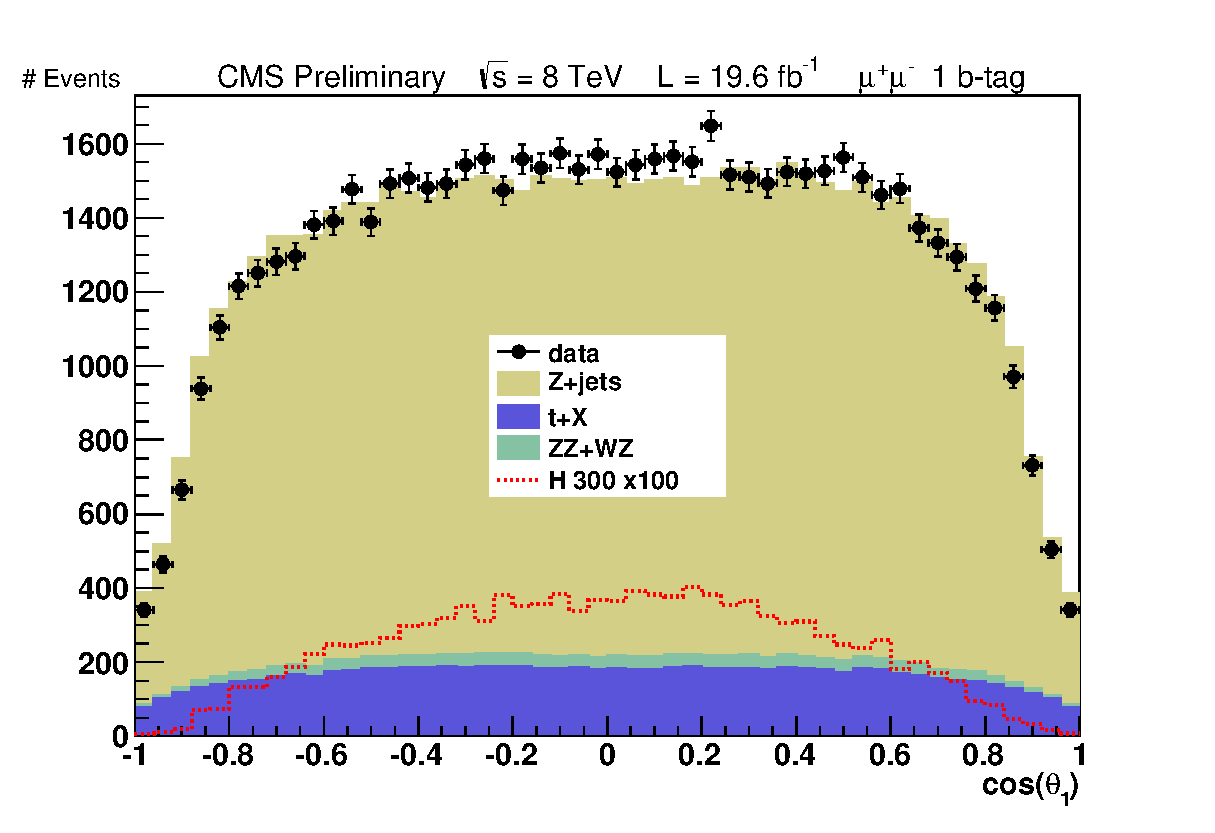
\includegraphics[width=0.33\textwidth]{presentation/defense/images/preselection/1/mu/costheta1.eps}
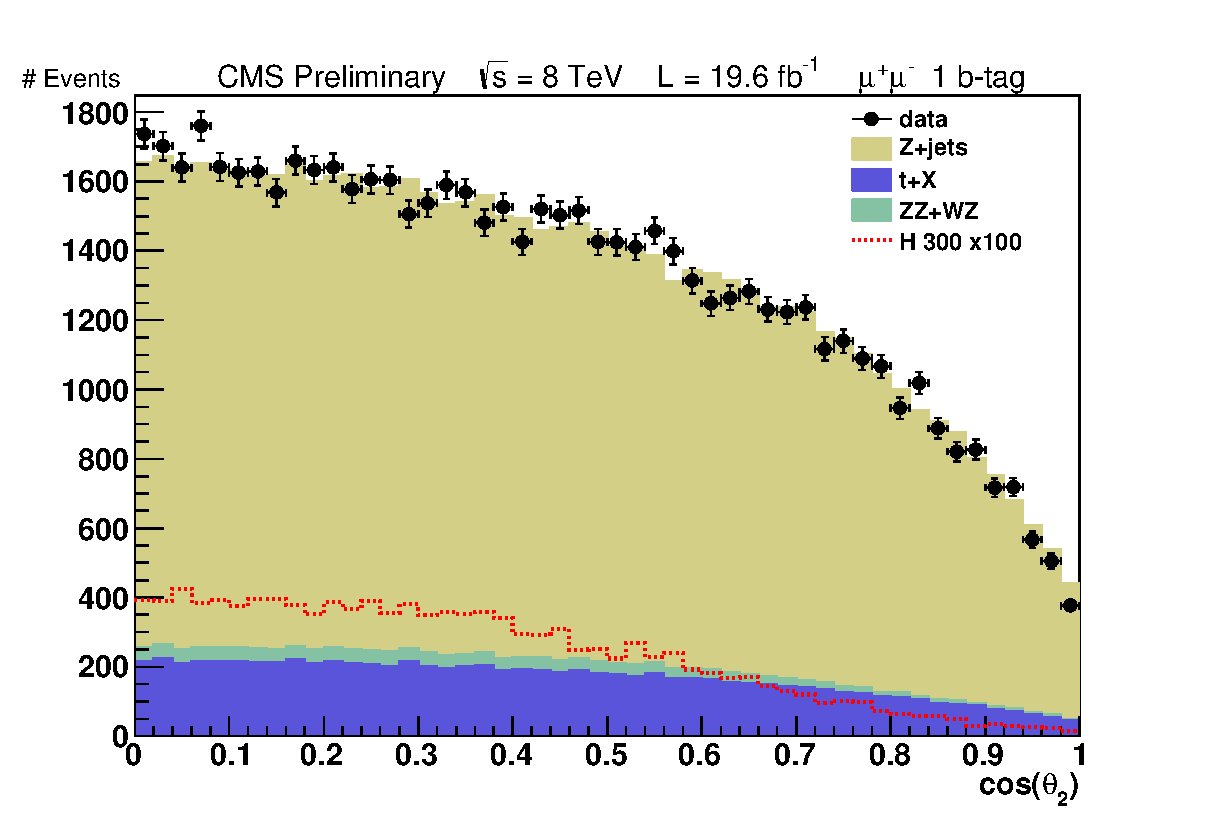
\includegraphics[width=0.33\textwidth]{presentation/defense/images/preselection/1/mu/costheta2.eps}
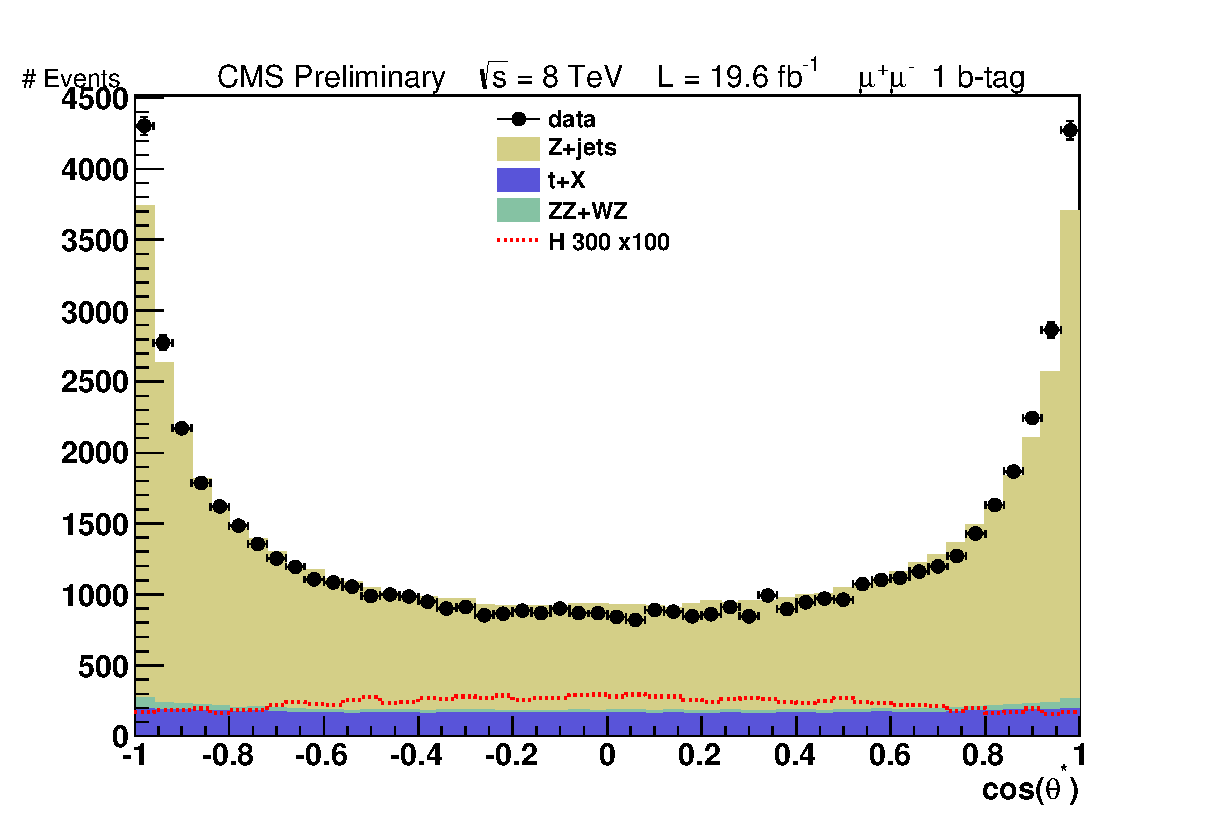
\includegraphics[width=0.33\textwidth]{presentation/defense/images/preselection/1/mu/costhetast.eps}
}
\centerline{
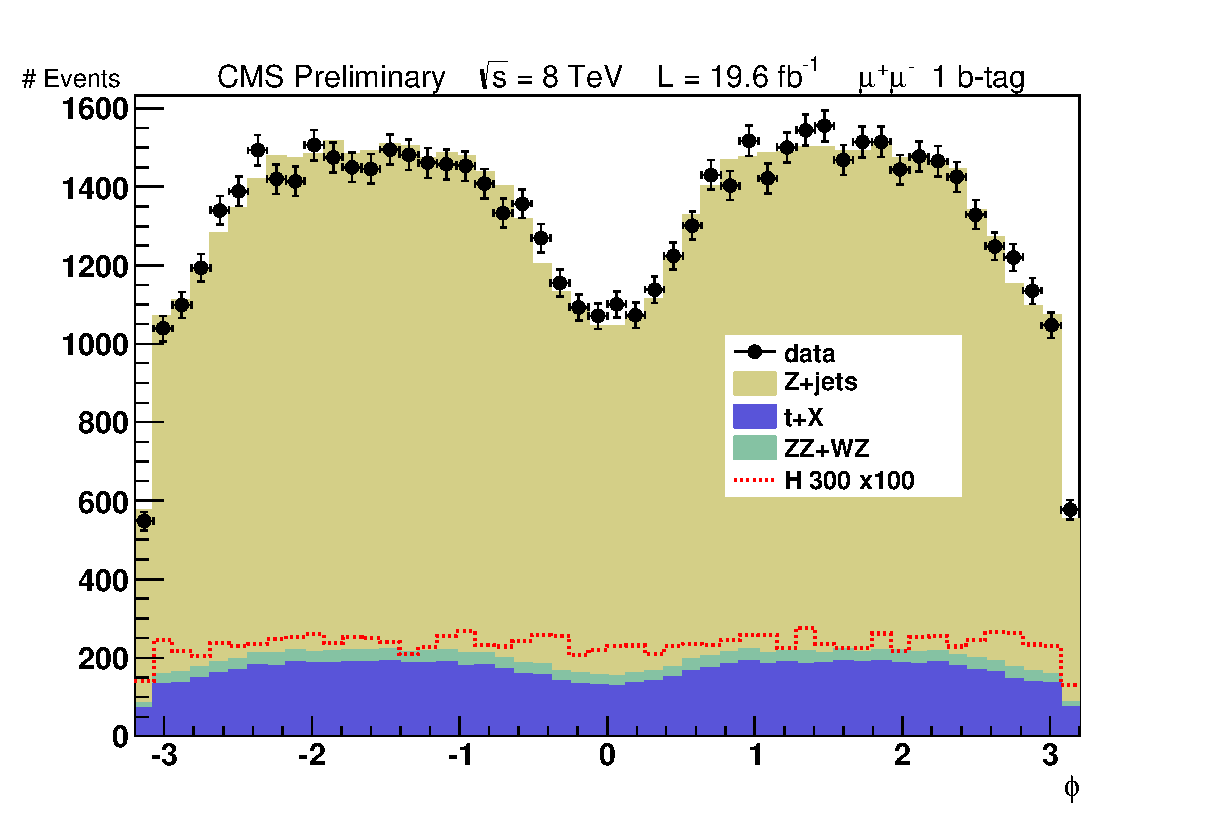
\includegraphics[width=0.33\textwidth]{presentation/defense/images/preselection/1/mu/phi.eps}
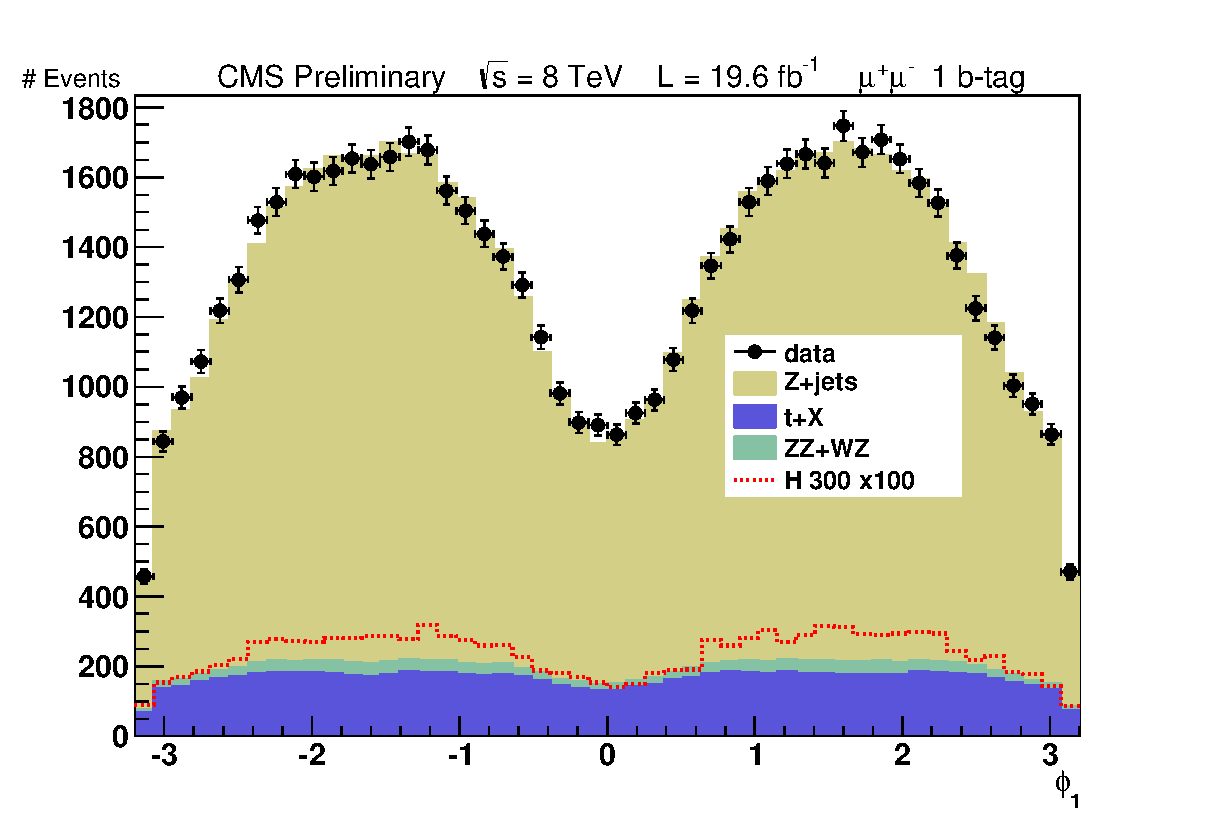
\includegraphics[width=0.33\textwidth]{presentation/defense/images/preselection/1/mu/phi1.eps}
}
\caption{
Five angular distributions of $\cos\theta_1, \cos\theta_2, \cos\theta^*, \Phi$, $\Phi_1$ and the helicity likelihood discriminant for 2012 muon data (points) and Summer 12 Monte Carlo samples (histogram) in the 1 b-tag category.  Open histograms indicate the expected distribution for a Higgs boson with mass 300 GeV. The selection is as described in preselection.
\label{helicityDistDataMCM1}}
\end{figure}
%%%%%%%%%%%%%
%%%%%%%%%%%%%
\begin{figure}[thb!]
\centerline{
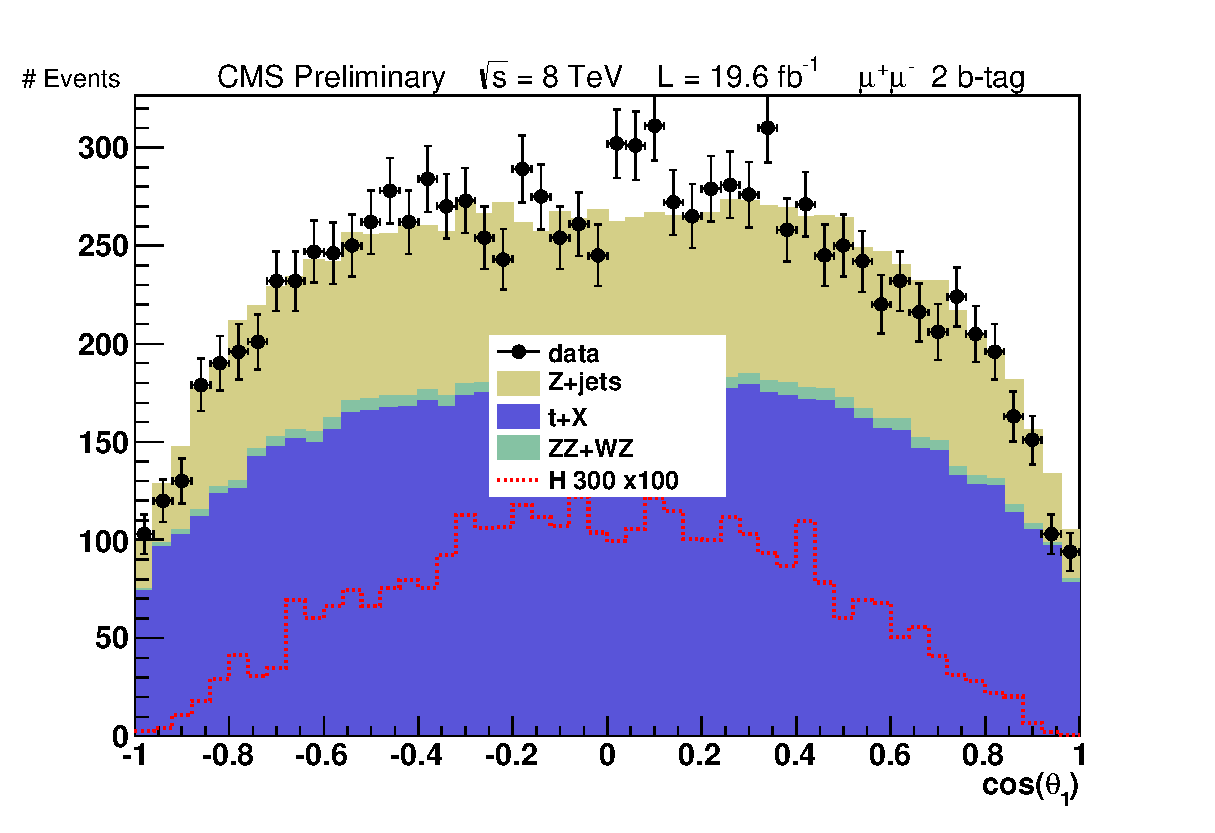
\includegraphics[width=0.33\textwidth]{presentation/defense/images/preselection/2/mu/costheta1.eps}
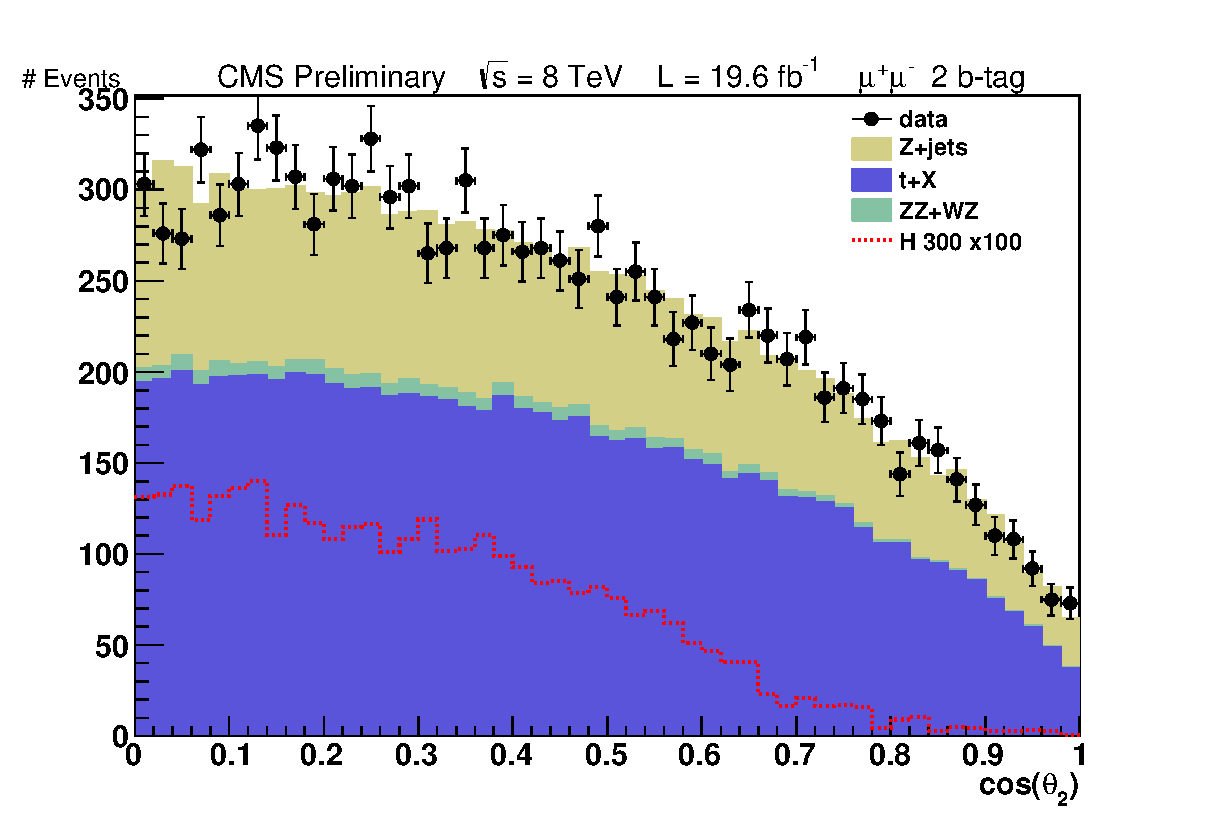
\includegraphics[width=0.33\textwidth]{presentation/defense/images/preselection/2/mu/costheta2.eps}
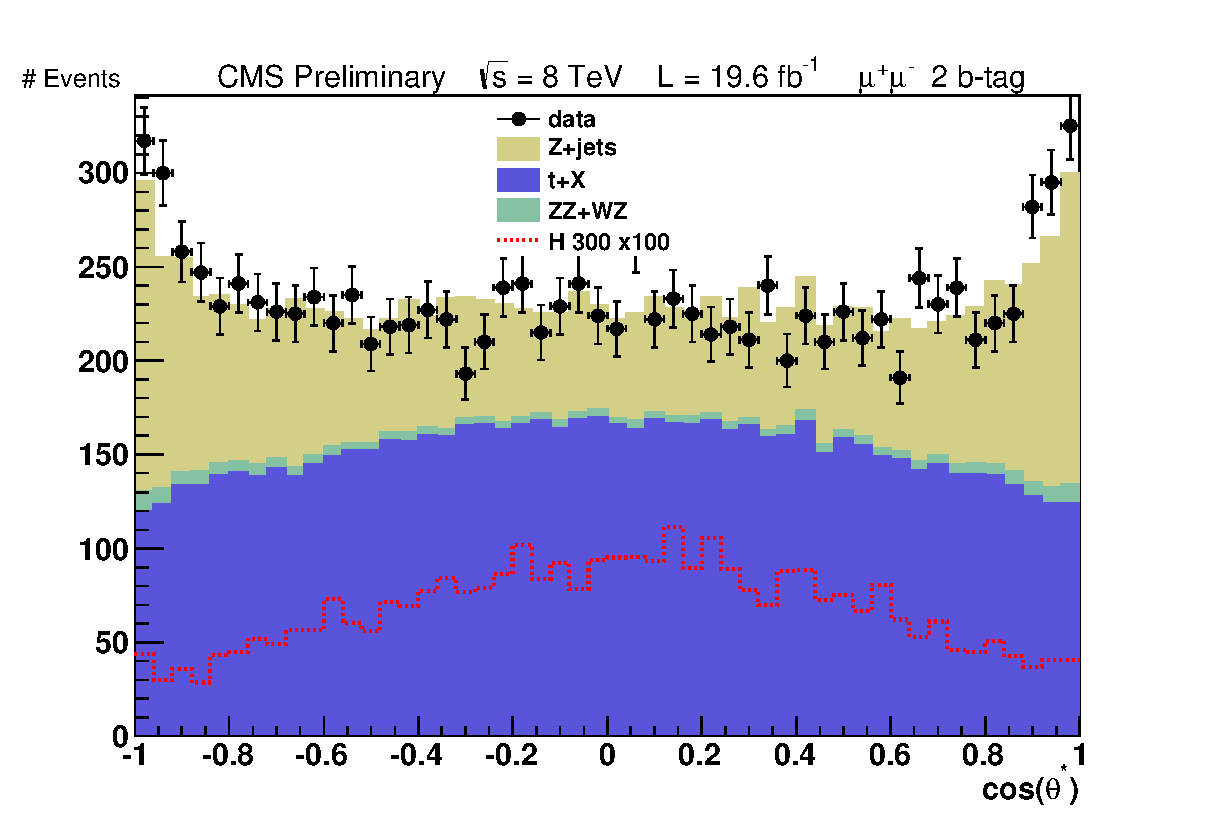
\includegraphics[width=0.33\textwidth]{presentation/defense/images/preselection/2/mu/costhetast.eps}
}
\centerline{
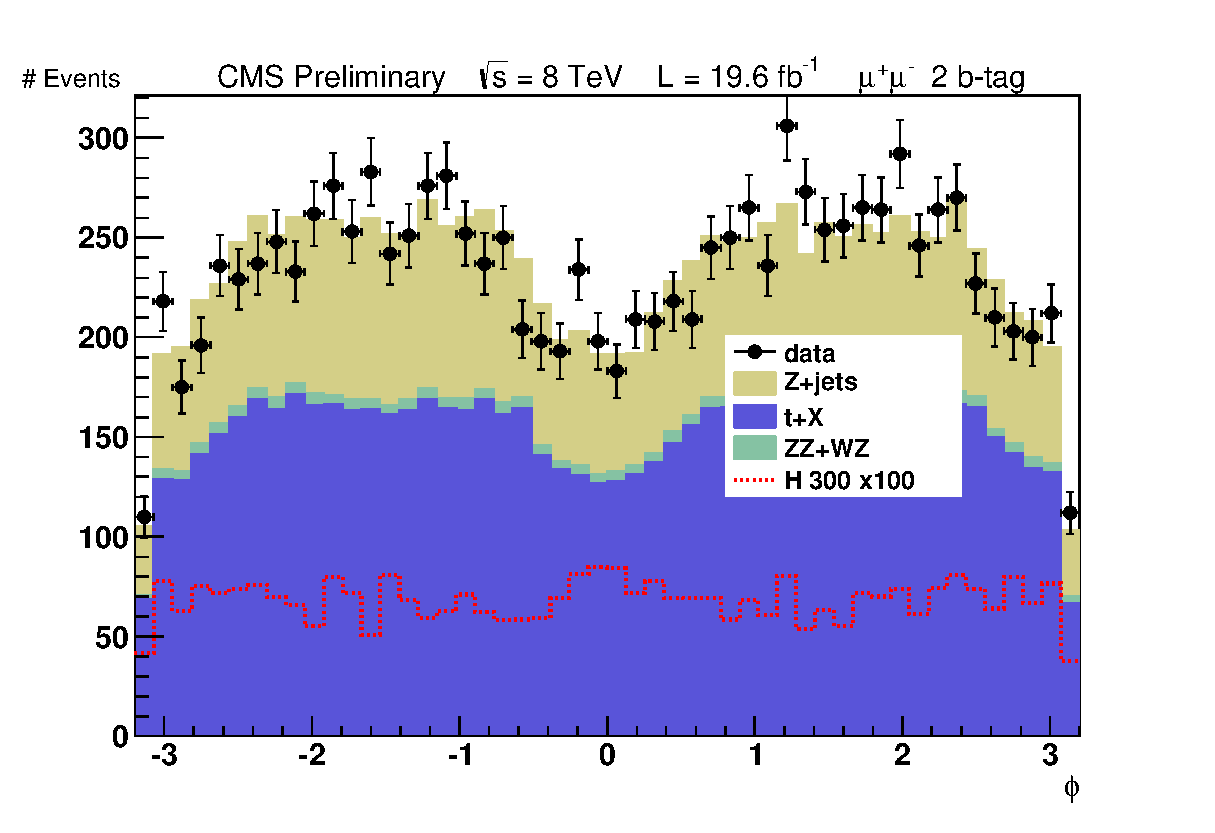
\includegraphics[width=0.33\textwidth]{presentation/defense/images/preselection/2/mu/phi.eps}
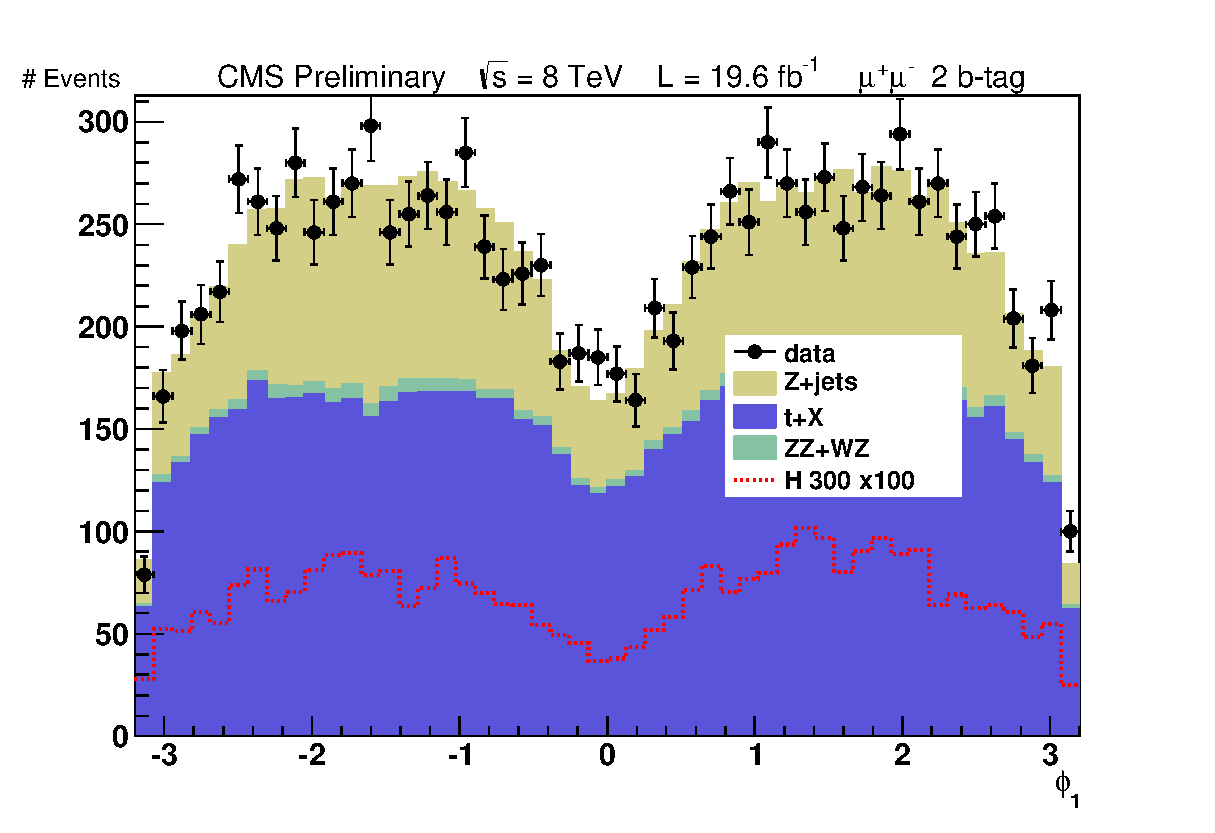
\includegraphics[width=0.33\textwidth]{presentation/defense/images/preselection/2/mu/phi1.eps}
}
\caption{
Five angular distributions of $\cos\theta_1, \cos\theta_2, \cos\theta^*, \Phi$, $\Phi_1$ and the helicity likelihood discriminant for 2012 muon data (points) and Summer 12 Monte Carlo samples (histogram) in the 2 b-tag category.  Open histograms indicate the expected distribution for a Higgs boson with mass 300 GeV. The selection is as described in preselection.
\label{helicityDistDataMCM2}}
\end{figure}
%%%%%%%%%%%%%

\subsection{Angular Discriminant}

The information from the angular variables in the final state particles can be used to define a likelihood discriminate.  This likelihood discriminate allows us to select the topology that is consistent with a Higgs decay.  The first step in creating the likelihood discriminate is to build the probability density functions  for both the signal and background events.  After these have been defined we use them to get a probability ratio as seen in Equation~\ref{eq:LD} where LD is the likelihood discriminant, $P_{sig}$ is the probability the candidate is signal, and $P_{BG}$ is the probability the candidate is background.
  \begin{equation} LD = \dfrac{P_{sig}}{P_{sig}+P_{BG}} \label{eq:LD}\end{equation}

This definition puts candidates that have a topology like the signal to have a LD value close to 1 and those candidates with a topology similar to those of the background will have a LD value closer to 0.  This allows us to use this LD variable (in the future referenced to as helyLD or helicity LD) for event selection by requiring candidates to have a value higher than a certain threshold.

The function $P_{sig}$ (Equation~\ref{eq:psig}) is defined as the ideal probability function~\cite{PhysRevD.81.075022} ($P_{ideal}$) multiplied by four 1D acceptance functions.  
\begin{equation} P_{sig} = P_{ideal}(\theta_1, \theta_2, \theta^*, \Phi, \Phi_1 ;M)G_{\theta_1}(\theta_1;M)G_{\theta_2}(\theta_2;M)G_{\theta^*}(\theta^*;M)G_{\Phi_1}(\Phi_1;M) \label{eq:psig}\end{equation}

In Equation~\ref{eq:psig} M is the mass of the reconstructed Higgs candidate and the acceptance functions ($G_{\theta_1},G_{\theta_2},G_{\theta^*},G_{\Phi_1}$) are empirically calculated by fitting the signal Monte Carlo Simulations.

Similar to data, the probability distribution function for background is given in Equation~\ref{eq:psigback}.
\begin{equation} P_{BG} = P_{\theta_1}(\theta_1;M)P_{\theta_2}(\theta_2;M)P_{\theta^*}(\theta^*;M)P_{\Phi_1}(\Phi_1;M)P_{\Phi^*}(\Phi^*;M) \label{eq:psigback}\end{equation}

Each probability function is obtained entirely empirically from the fits to the simulation background Monte Carlo samples.

The acceptance functions are created for each angular variable through a number of steps.  First we define a number of bins around a central Higgs mass that we are looking at.  Then, using signal samples in these bins, we fit each angular variable to a polynomial.  The list of polynomials can be seen in Table~\ref{tab:poly}.  An example fitting for the acceptance functions a reconstructed Higgs mass of 500 GeV can be seen in Figure~\ref{fig:500fit}.
%%%%%%%%%%%%%%%%%%%%%%%%%%%%%%%%%
\begin{center}
\begin{table}[htb]
\caption{%
  \small The polynomials used for fitting each angular variable.%
}
\begin{center}
\begin{tabular}{ c c }
Variable  & Polynomial \\ \hline
$\cos(\theta_1)$ & $a_2 x^2+a_4 x^4$ \\
$\cos(\theta_2)$ & $a_2 x^2+a_4 x^4$ \\
$\cos(\theta^*)$ & $a_2 x^2+a_4 x^4+a_6 x^6$\\
$\Phi$ &   $1 + a_0 cos(x) + a_1 cos(2x)$\\
$\Phi_1$ & $1 + a_0 cos(x) + a_1 cos(2x);$ \\
\end{tabular}
\end{center}
\label{tab:poly}
\end{table}
\end{center}
%%%%%%%%%%%%%%%%%%%%%%%%%%%%%%%%
%%%%%%%%%%%%
\begin{figure}[htb!]
\begin{center}
\centerline{
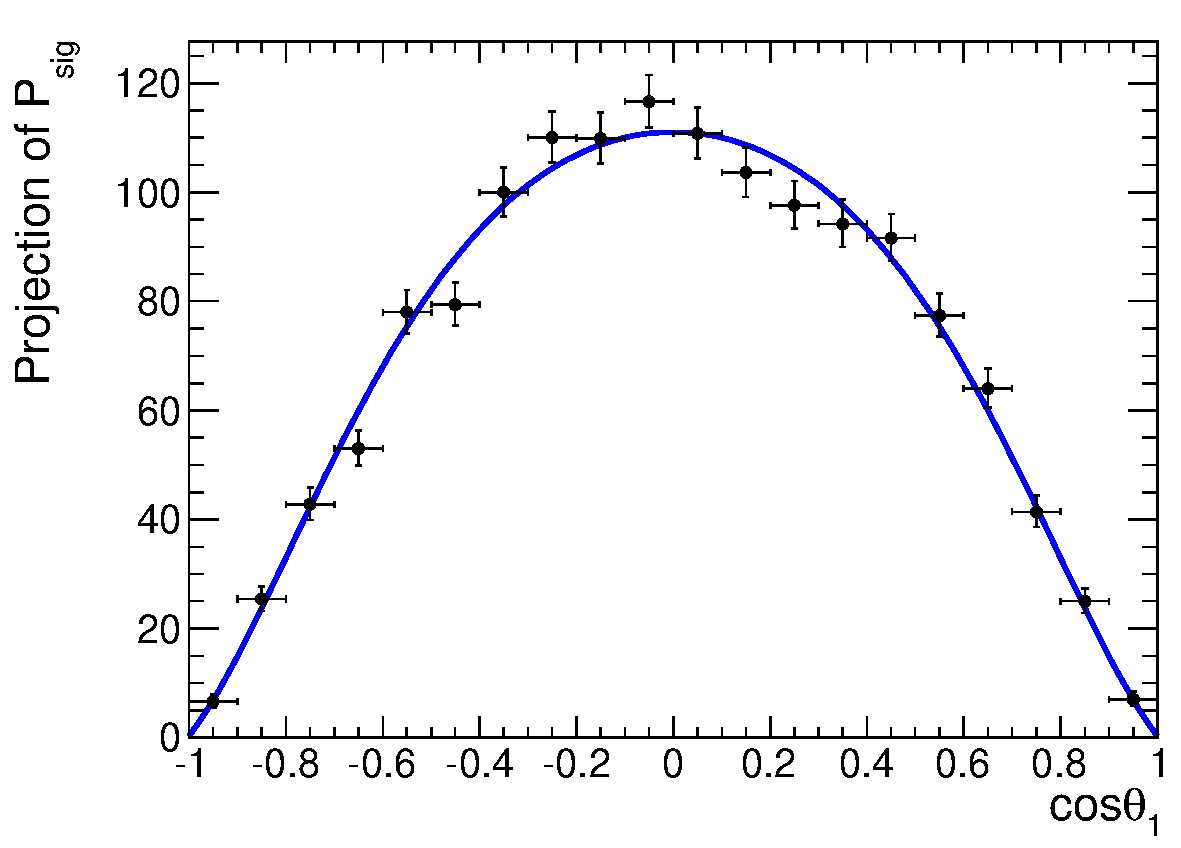
\includegraphics[width=0.33\textwidth]{presentation/defense/images/plots/sigPDF_CosTheta1proj_500.pdf}
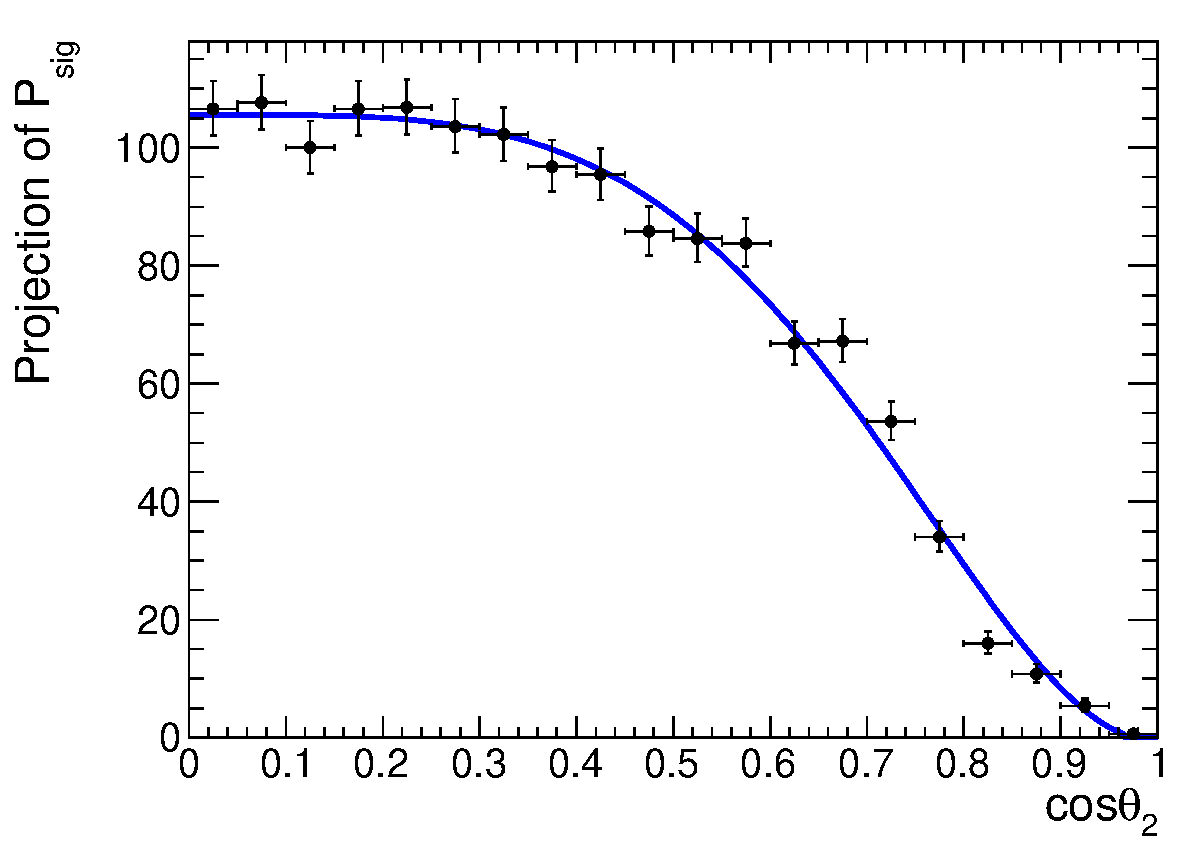
\includegraphics[width=0.33\textwidth]{presentation/defense/images/plots/sigPDF_CosTheta2proj_500.pdf}
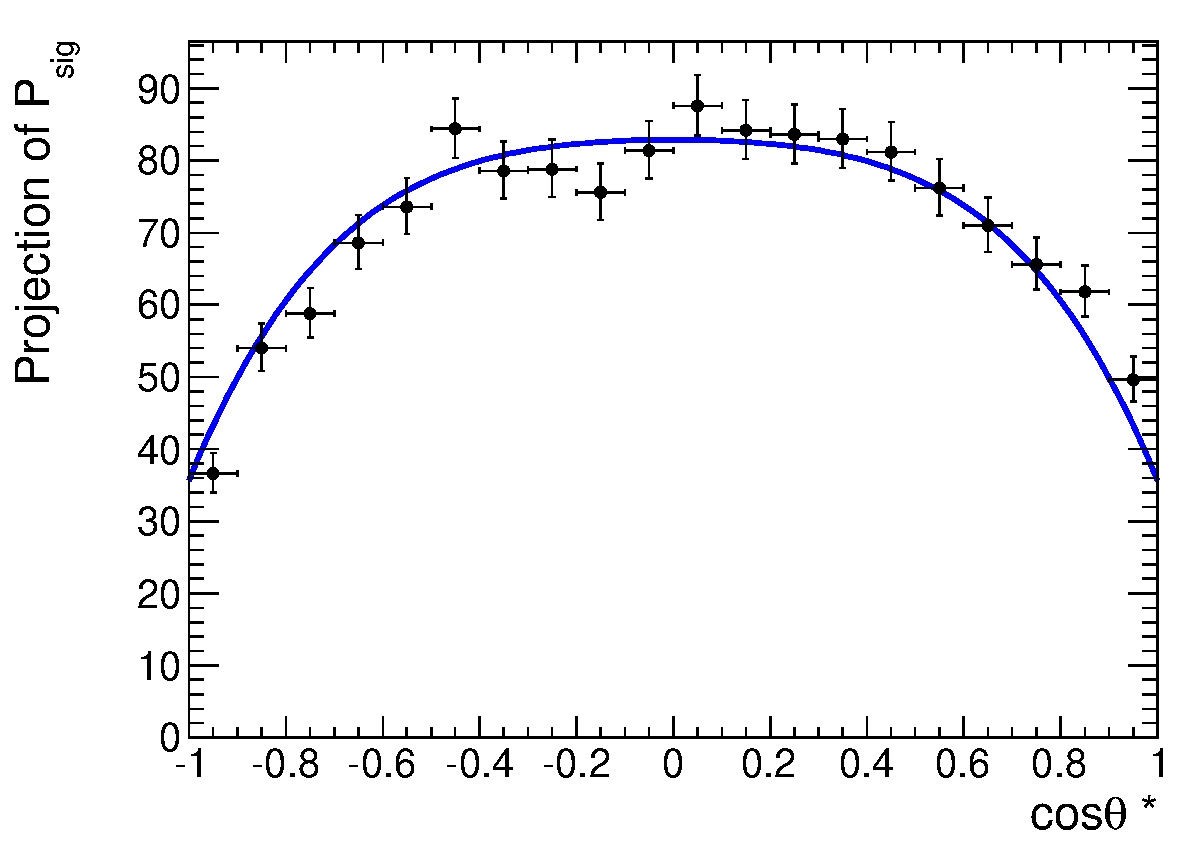
\includegraphics[width=0.33\textwidth]{presentation/defense/images/plots/sigPDF_CosThetaSproj_500.pdf}
}
\centerline{
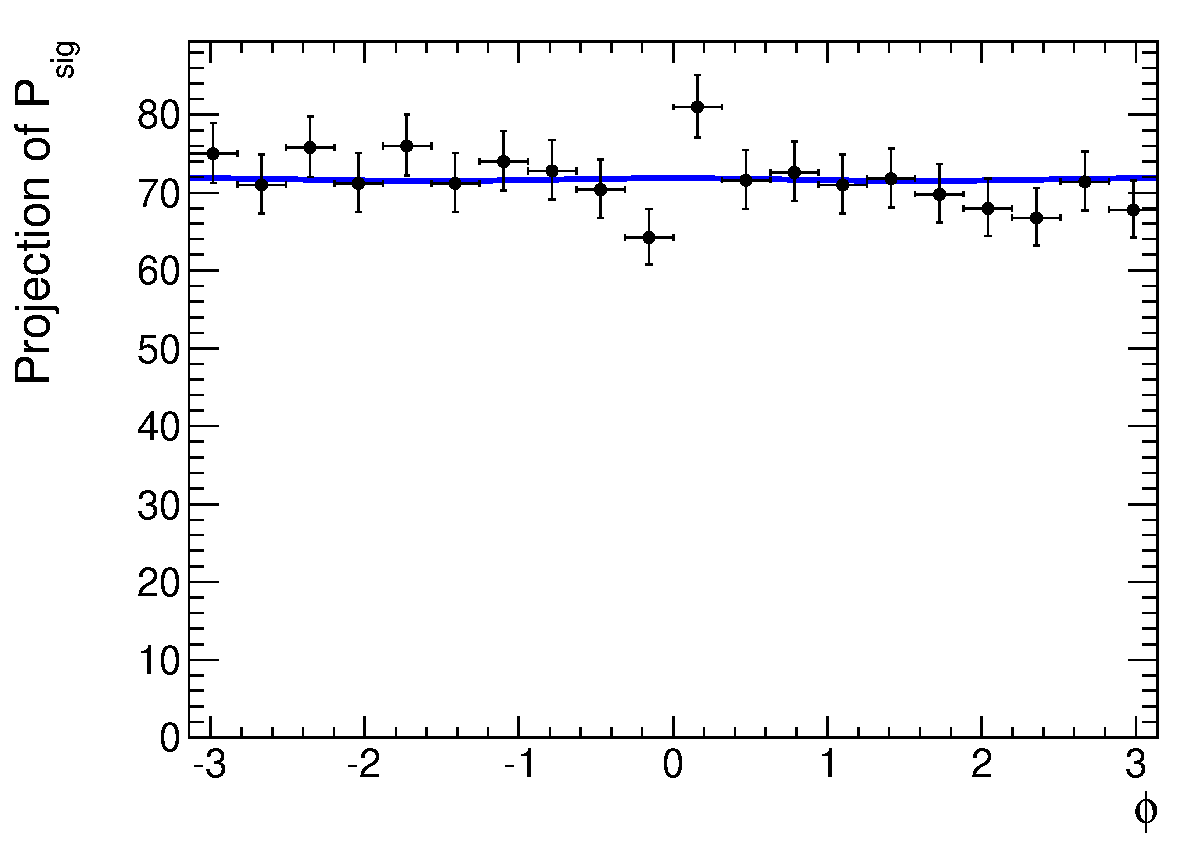
\includegraphics[width=0.33\textwidth]{presentation/defense/images/plots/sigPDF_Phiproj_500.pdf}
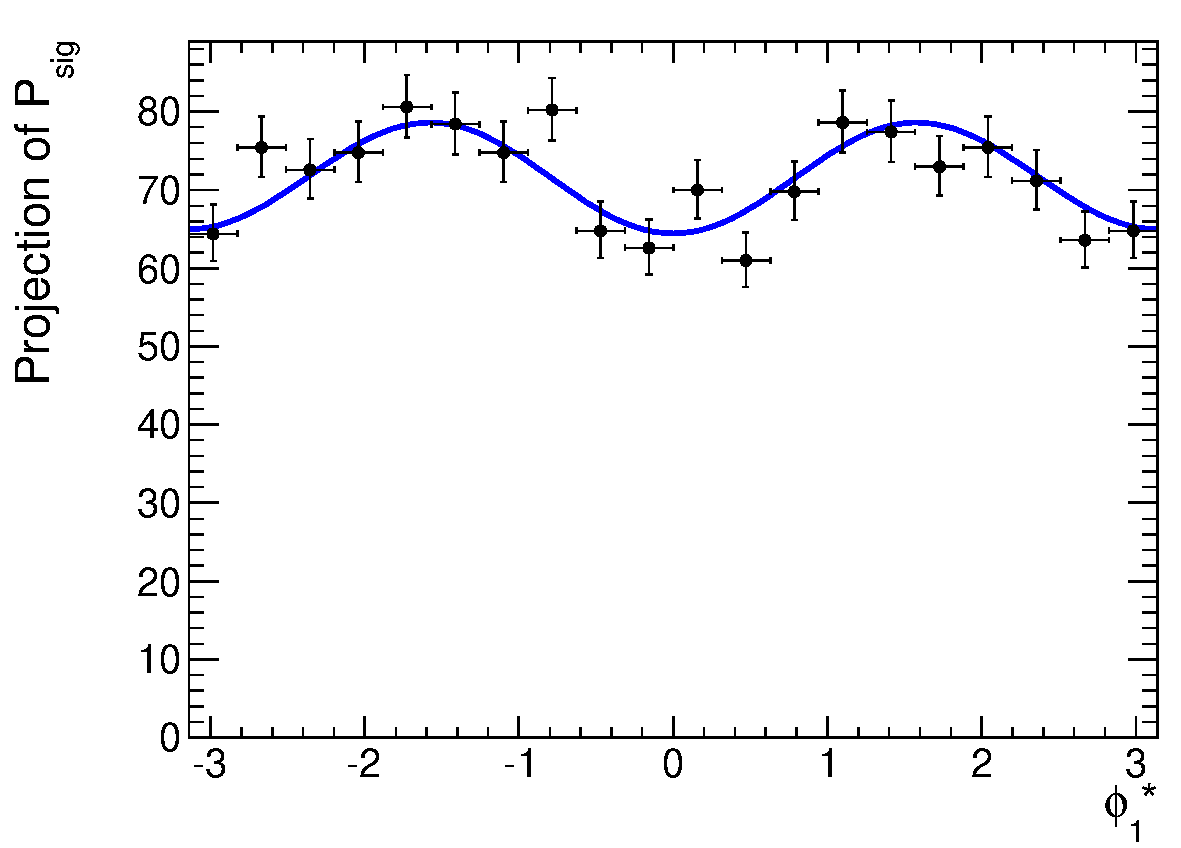
\includegraphics[width=0.33\textwidth]{presentation/defense/images/plots/sigPDF_PhiStar1proj_500.pdf}
}
\centerline{
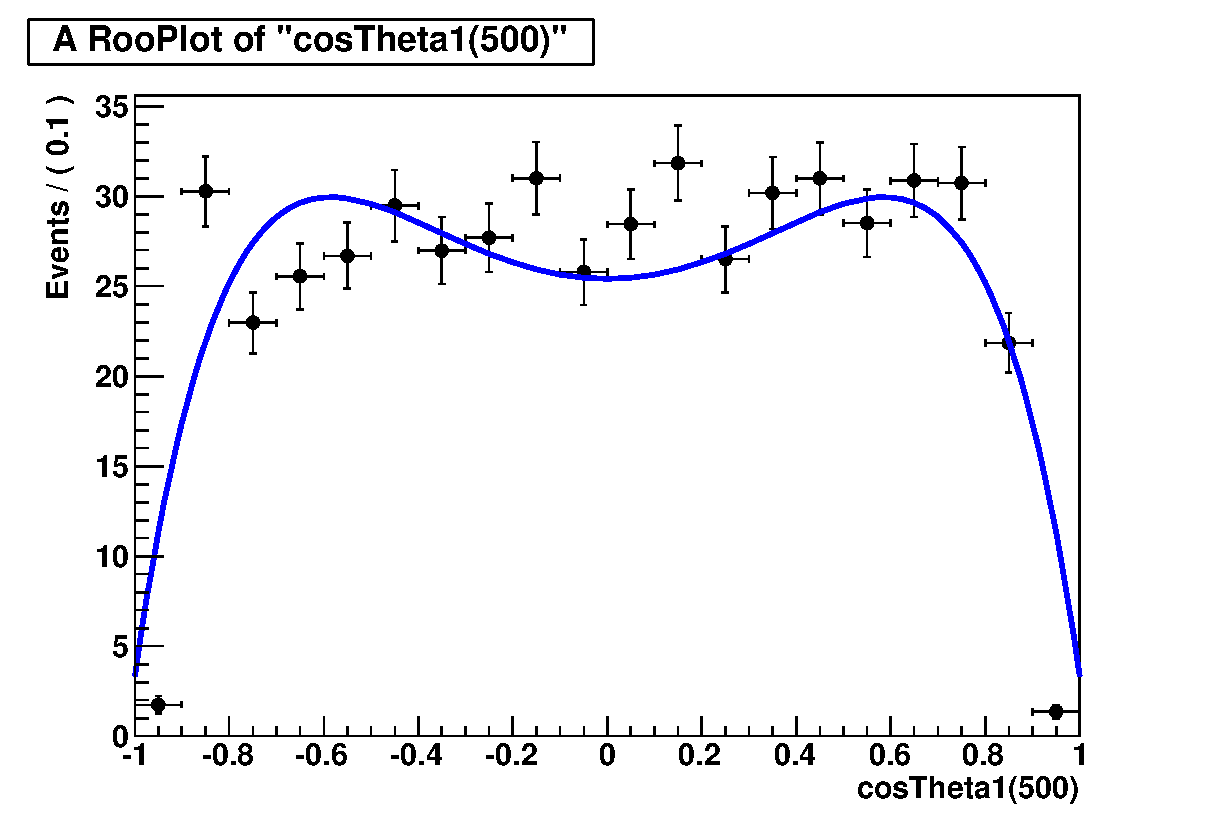
\includegraphics[width=0.33\linewidth]{Optimization/poly_fit/costheta1/500.eps}
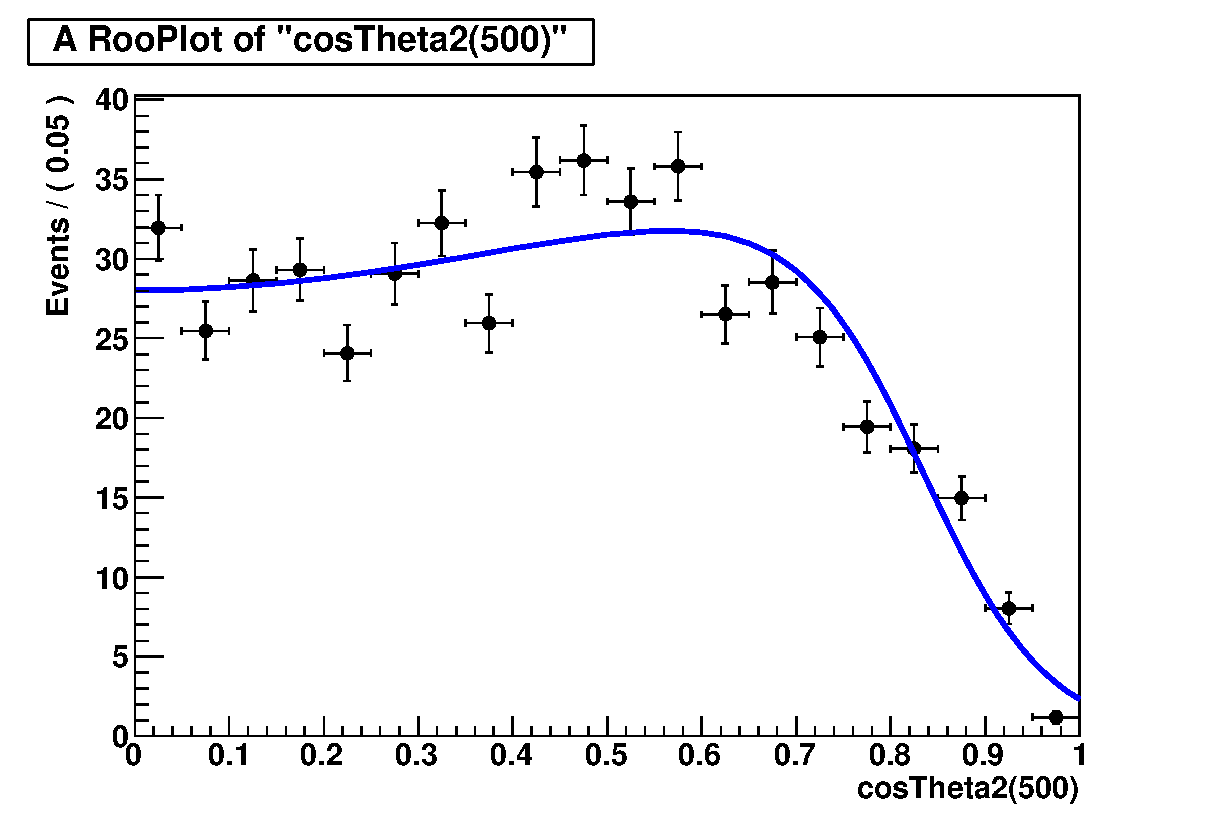
\includegraphics[width=0.33\linewidth]{Optimization/poly_fit/costheta2/500.eps}
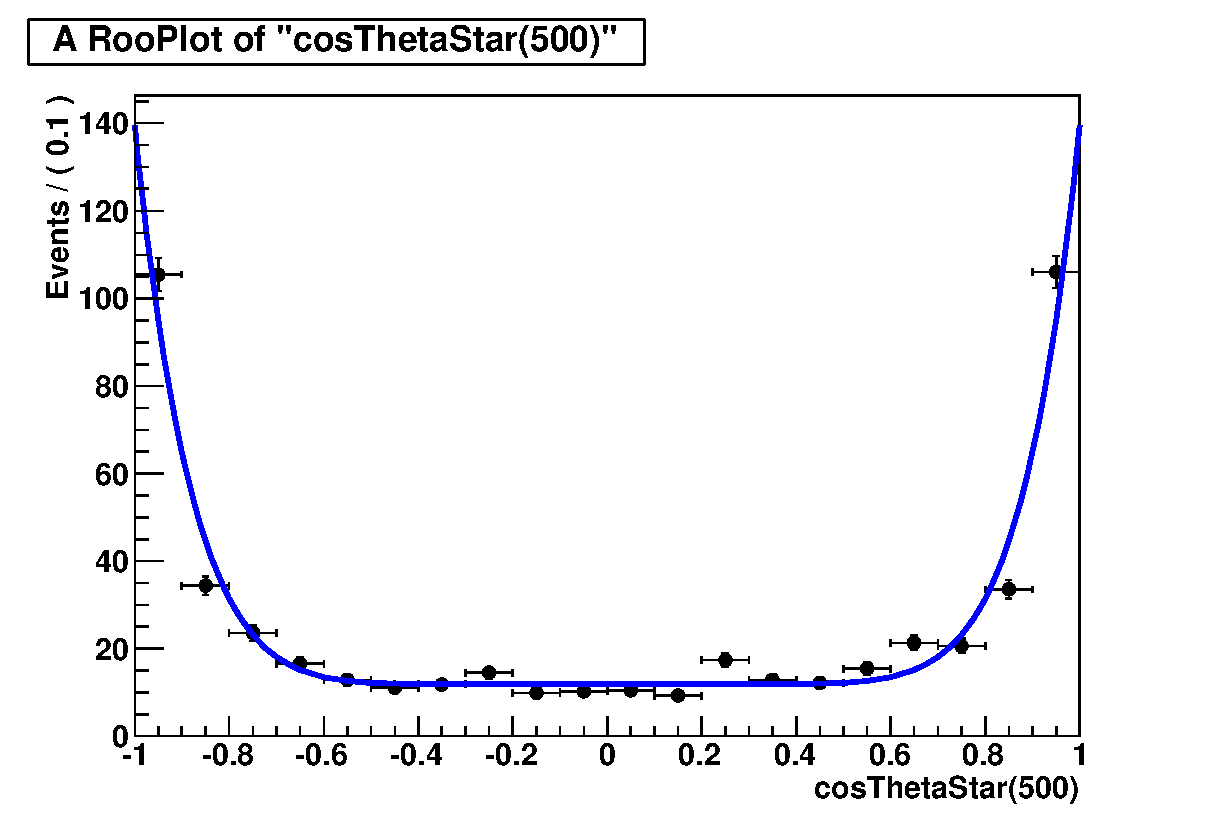
\includegraphics[width=0.33\linewidth]{Optimization/poly_fit/costhetastar/500.eps}
}
\centerline{
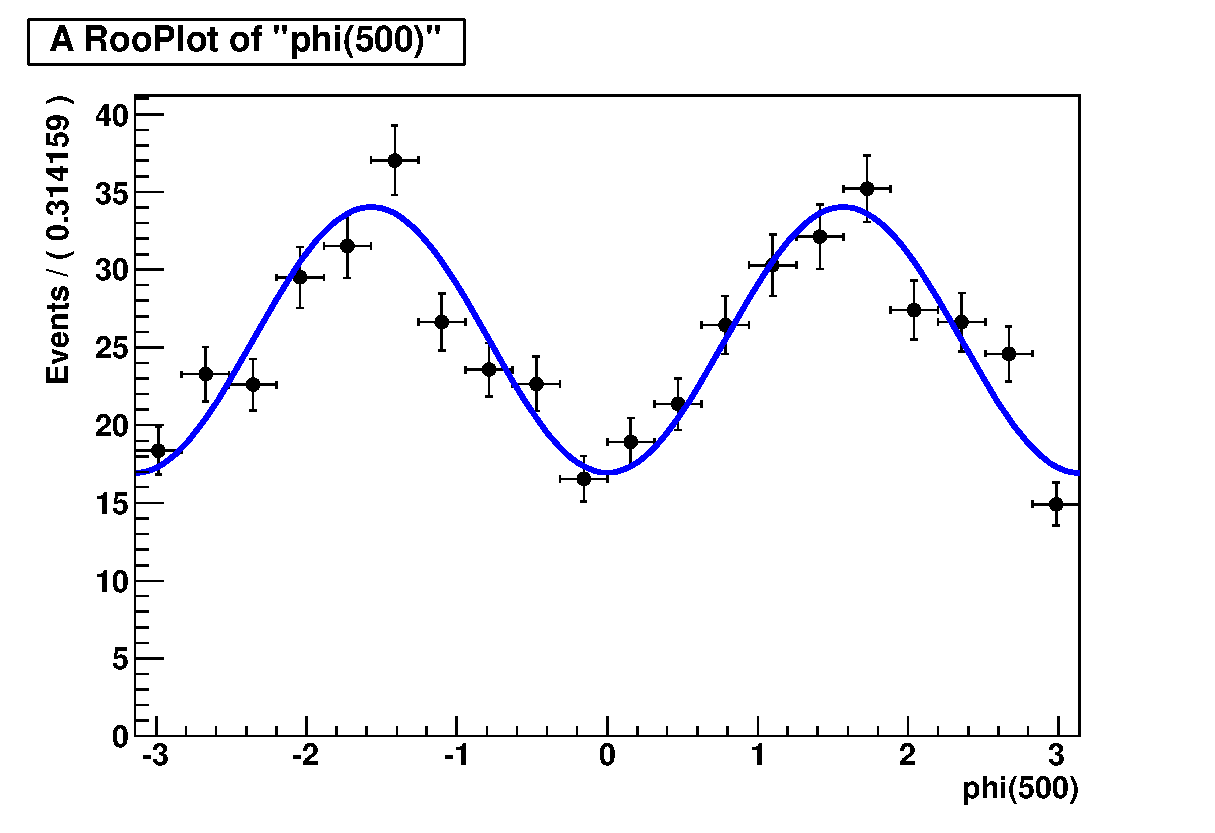
\includegraphics[width=0.33\linewidth]{Optimization/poly_fit/phi/500.eps}
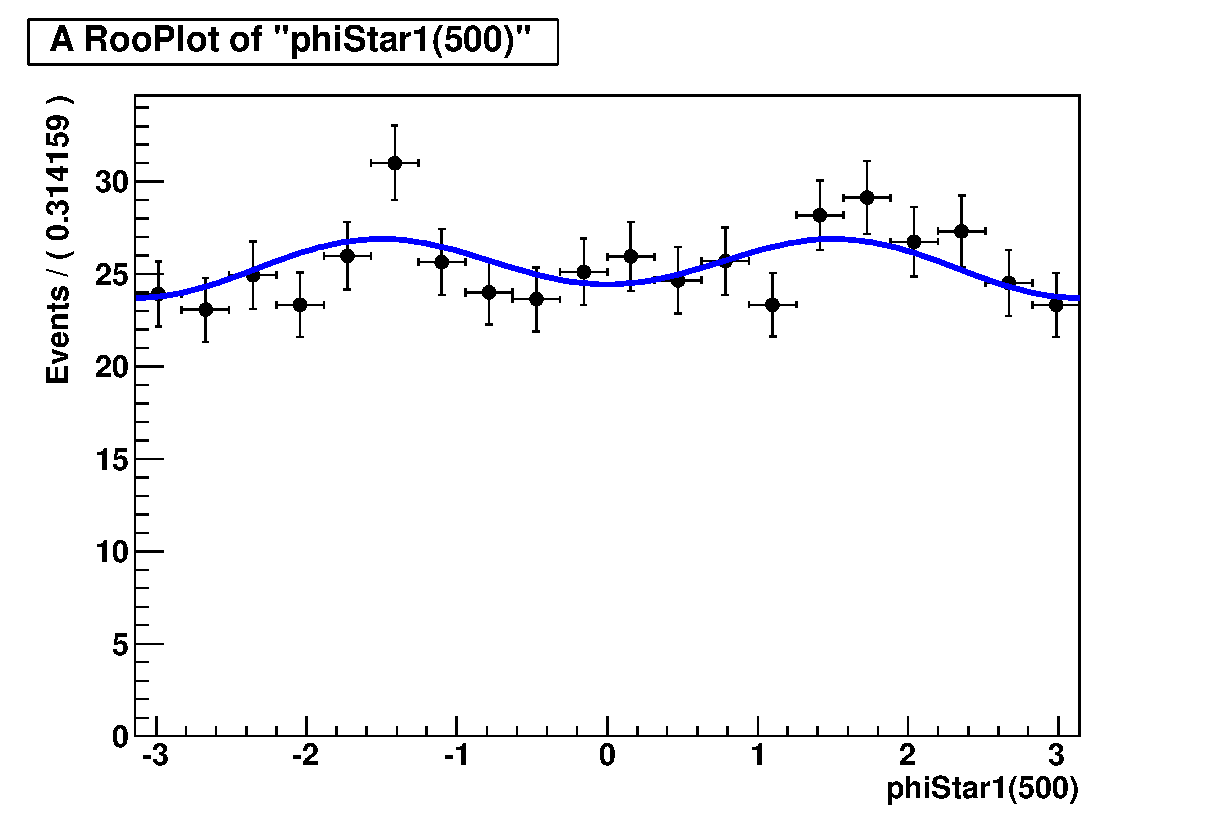
\includegraphics[width=0.33\linewidth]{Optimization/poly_fit/phi1/500.eps}
}
\caption{
Fitting the angular variables for a reconstructed Higgs mass of 500 GeV in signal Monte Carlo samples(first 5 plots) and for the Z+Jets background samples (bottom 5 plots). These are taken in a mass window of 450 GeV to 550 GeV in the ZZ invariant mass distribution.
}
\label{fig:500fit}
\end{center}
\end{figure}
%%%%%%%%%%%%

After the polynomials are fit for the range of reconstructed Higgs masses coefficients of the polynomials are then fit with a polynomial to parameterize the fits as a function of the ZZ invariant mass. This allows the acceptance functions to be a function of only the ZZ invariant mass and extends the function to be continuous for the Higgs mass values that we do not have Monte Carlo simulations for.  An example of calculating the parameters can be seen in Figure~\ref{fig:fit_poly} for $\cos(\theta_1)$.  Similar fitting is done for the other angular variables.  Figure~\ref{fig:fit_param} shows the differences for the acceptance function $G_{\theta^*}(\theta^*;450)$ between a direct fit and using the extrapolation used to get the parameritization of the polynomial coefficients.


%%%%%%%%%%%%
\begin{figure}[htb!]
\begin{center}
\centerline{
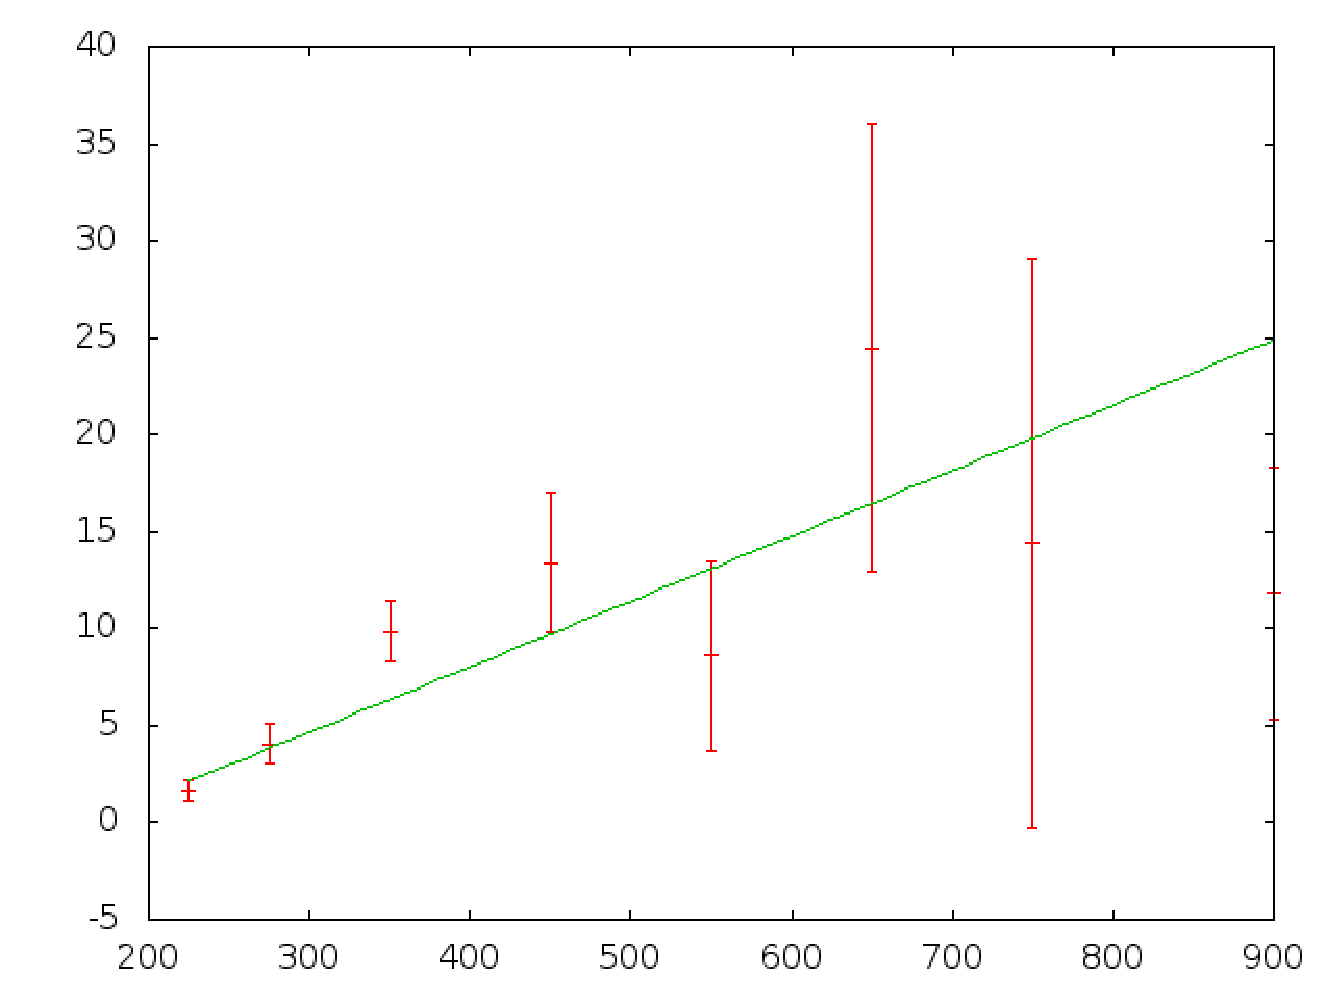
\includegraphics[width=0.33\textwidth]{Optimization/a2.pdf}
\includegraphics[width=0.33\textwidth]{Optimization/a4.pdf}
\includegraphics[width=0.33\textwidth]{Optimization/a6.pdf}
}
\caption{
Fitting the parameters $a_2$ (left), $a_4$ (middle), $a_6$ (right) for $\cos(\theta_1)$ to calculate the acceptance function $G_{\theta_1}(\theta_1;M)$ as a function of the reconstructed Higgs mass.  The same fitting is done for the other angular variables.
}
\label{fig:fit_poly}
\end{center}
\end{figure}
%%%%%%%%%%%%

%%%%%%%%%%%%
\begin{figure}[htb!]
\begin{center}
\centerline{
\includegraphics[width=0.49\textwidth]{Optimization/costhetast_450_fit.pdf}
\includegraphics[width=0.49\textwidth]{Optimization/costhetast_450_extrap.pdf}
}
\caption{A $\cos(\theta^*)$ comparison for the 450 GeV reconstructed Higgs mass signal simulations fitting the  acceptance function $G_{\theta_1}(\theta_1;M)$ directly to data (right), and plotting $G_{\theta_1}(\theta_1;450)$ from the extrapolated polynomial coefficients (left). There is very good agreement between the fitting and extrapolation.  
}
\label{fig:fit_param}
\end{center}
\end{figure}
%%%%%%%%%%%%

With these functions defined, we can then calculate the helicity likelihood discriminant as a function of the ZZ invariant mass.  Figure~\ref{fig:hely_LD} shows the distributions for the HelyLD in the 2012 data for both electrons and muons as well as an example of the shape of signal for a Higgs mass of 300 GeV.  This is shown for each of the 3 b-tag regions.  We can see that particularly in the 0-tag and 1-tag regions this is a powerful discriminating variable for the Z+Jets background.  In the 2-tag region the $\Pqt \Paqt$ background is much more prevalent, but this selection is still powerful against the Z+Jets.  


%%%%%%%%%%%%
\begin{figure}[htb!]
\begin{center}
\centerline{
\includegraphics[width=0.45\textwidth]{presentation/defense/images/preselection/0/el/helyLD.eps}
\includegraphics[width=0.45\textwidth]{presentation/defense/images/preselection/0/mu/helyLD.eps}
}
\centerline{
\includegraphics[width=0.45\textwidth]{presentation/defense/images/preselection/1/el/helyLD.eps}
\includegraphics[width=0.45\textwidth]{presentation/defense/images/preselection/1/mu/helyLD.eps}
}
\centerline{
\includegraphics[width=0.45\textwidth]{presentation/defense/images/preselection/2/el/helyLD.eps}
\includegraphics[width=0.45\textwidth]{presentation/defense/images/preselection/2/mu/helyLD.eps}
}
\caption{
HelyLD for electrons (right) and muons(left) for the 3 b-tag categories, 0-tag (top), 1-tag (middle), 2-tag (bottom). The preselection is applied to this data and the 300 GeV signal Monte Carlo is scaled by 100 to get a better picture of the comparison.
}
\label{fig:hely_LD}
\end{center}
\end{figure}
%%%%%%%%%%%%


There is a discrepancy between the data and Monte Carlo simulated samples, in that the data is more background like than simulation suggests. This is caused by the simulated Z+Jets samples not correctly representing data in the $\cos(\theta^*)$ samples.  This discrepancy can be seen in Figure~\ref{fig:costhetast} and is in the range of 0.8 $< |\cos(\theta^*)| <$ 1.0.  If we keep only events in which $|\cos(\theta^*)| <$ 0.8 then the HelyLD distribution between data and simulation is within good agreement, as can be seen in Figure~\ref{fig:helyld_cut_costhetast}.  Similar studies have been done scaling the simulation to data resulting in a correction of the HelyLD distribution.  While these measures will correct the distribution, this region of disagreement is rejected from the analysis later and there is no significant difference on the final yields between correcting the $\cos(\theta^*)$ distribution or not. Because of these reasons we do not apply any corrections to the HelyLD distribution.


%%%%%%%%%%%%
\begin{figure}[htb!]
\begin{center}
\centerline{
\includegraphics[width=0.45\textwidth]{presentation/defense/images/preselection/el/costhetast.eps}
\includegraphics[width=0.45\textwidth]{presentation/defense/images/preselection/mu/costhetast.eps}
}
\caption{$\cos(\theta^*)$ distributions for electrons (right) and muons (left). The mismatch between simulation an data can be seen in the range 0.8 $< |\cos(\theta^*)| <$ 1.0. 
}
\label{fig:costhetast}
\end{center}
\end{figure}
%%%%%%%%%%%%
%%%%%%%%%%%%
\begin{figure}[htb!]
\begin{center}
\centerline{
\includegraphics[width=0.45\textwidth]{presentation/defense/images/costhetast_cut/el/helyLD.eps}
\includegraphics[width=0.45\textwidth]{presentation/defense/images/costhetast_cut/mu/helyLD.eps}
}
\caption{HelyLD distribution after applying the selection 0.8 $< |\cos(\theta^*)|$ showing much better agreement between Monte Carlo simulation and data.
}
\label{fig:helyld_cut_costhetast}
\end{center}
\end{figure}
%%%%%%%%%%%%




%\section{Neural Network}
%\label{sec:NN}

%=================================================================
\section{Signal Optimization Based on Helicity Neural Network}
The Helicity LD is such an important part of the analysis that a cross check on its performance is performed.  For this a Neural Network is applied to separate Higgs signal from background using the five helicity angles of the final objects in the analysis as inputs. A training and test evaluation has been performed with the framework of the TMVA package~\cite{tmva} using the true event weight mix of Monte Carlo processes as background and Higgs Monte Carlo. Both the training and testing samples for both background and signal are constructed and events randomly mixed outside of the Neural Network.  There are 37,874 signal events and 38,378 background events evenly split between testing and training.  The Neural Network was trained on the Monte Carlo simulation generated for a hypothetical Higgs mass of 400 GeV. This training was on events that passed the previously explained preselection and the $Z$ boson mass window selection, but before the selection on MET significance which will be examined in more detail later in this section.


\subsection{Neural Network Architecture}
The architecture of the Neural Network consists of two hidden layers with N and N neurons respectively, where N is the number of variables, and one output node as shown in Figure ~\ref{fig:NNarch}.



%%%%%%%%%%%%
\begin{figure}[htb!]
\begin{center}
\centerline{
\includegraphics[width=0.6\linewidth]{Optimization/plots/NN/nn_network_architecture.pdf}
}
\caption{
Neural Network architecture used for the training.
}
\label{fig:NNarch}
\end{center}
\end{figure}
%%%%%%%%%%%%


\subsection{Helicity Neural Network}
The training and testing of the Neural Network can bee seen in Figure~\ref{fig:NNOutput}.  While there is separation between the signal and background and good agreement between testing and training, there is a definite spike in background at the same place as the signal spikes in the MLP (Multilayer perceptron neural network) training. The training was done with Monte Carlo generated for a hypothetical Higgs mass of 400 GeV, but then applied to the Monte Carlo for hypothetical Higgs masses of 300, 400, 500, and 600 GeV. This is because the angular components should not depend on Higgs mass. The distribution for all b-tag regions and multiple signal simulated samples can be seen in Figure~\ref{fig:0tag_mlp}, showing good discrimination between signal and background as well as good performance of the single 400 GeV training on the various signal samples.

%%%%%%%%%%%%
\begin{figure}[htb!]
\begin{center}
\centerline{
\includegraphics[width=0.8\linewidth]{Optimization/MLP.eps}
}
\caption{
The training is done after preselection and mixing electrons and muons.  Additionally we require at least one JP medium jet with training 400 GeV Higgs boson with a MLP neural network.
}
\label{fig:NNOutput}
\end{center}
\end{figure}
%%%%%%%%%%%%


%%%%%%%%%%%%
\begin{figure}[htb!]
\begin{center}
\centerline{
\includegraphics[width=0.8\linewidth]{Optimization/MLP_el.eps}
}
\centerline{
\includegraphics[width=0.8\linewidth]{Optimization/MLP_mu.eps}
}
\caption{
The MLP neural network distribution for electrons (top) and muons (bottom).  This training was done on the 400 GeV signal simulations, but applied to the 300, 400, 500, and 600 GeV samples to show the good agreement even training with only one sample.  The signal simulations are scaled for ease of reading.
}
\label{fig:NNOutput}
\end{center}
\end{figure}
%%%%%%%%%%%%

In addition to the MLP neural network, a Likelihood discriminant was calculated using the TMVA package to check the MLP performance using the same input parameters.  Figure~\ref{fig:windowcuts} shows the receiver operating characteristic (ROC) curve for the Helicity LD, MLP, and Likelihood discriminators. These show that when looking at the performance between the three after preselection requirements the MLP performs significantly better than the Helicity LD. However, after looking in windows of -6\%/+10\% around the generated Higgs mass we see the improvement drop away and we get very similar performance.  This shows that the MLP is training on additional information than the Helicity LD is using, but that this information is correlated to the mass of the reconstructed Higgs candidate.  


%%%%%%%%%%%%
\begin{figure}[htb!]
\begin{center}
\centerline{
\includegraphics[width=0.49\linewidth]{Optimization/pretag_ROC_full_5.eps}
\includegraphics[width=0.49\linewidth]{Optimization/pretag_ROC_win_5.eps}
}
\caption{The ROC curve for signal and background comparing the HelyLD, MLP, and an alternate training for a Likelihood Discriminant using the TMVA package after preselection (right).  The same curve is given with additional selection of -6\%/+10\% of the Higgs mass to give a better estimation of performance for the final shape analysis.
}
\label{fig:windowcuts}
\end{center}
\end{figure}
%%%%%%%%%%%%

In the 0-tag region the separation between signal and background looks similar to the training for Higgs 300, 400, and 500 GeV, but does not have much discrimination power for a Higgs of 200 GeV.  The discrimination power is virtually the same after applying an additional selection of -6\%/+10\% of the Higgs mass for all four cases. When comparing background rejection versus signal efficiency between the neural network and likelihood discriminate, the performance is for all practical purposes the same.

In the 1-tag region the separation between signal and background looks similar to the training for Higgs 300, 400, and 500 GeV, but does not have much discrimination power for a Higgs of 200 GeV.  The discrimination power is virtually the same after applying an additional selection of -6\%/+10\% of the Higgs mass for all four cases. When comparing background rejection versus signal efficiency between the neural network and likelihood discriminate the performance is for all practical purposes the same. See Figure~\ref{fig:nn_1tag_ROC}.

In the 2-tag region, after applying a selection of -6\%/+10\% of the Higgs mass, the discriminating power of the neural network is similar to the 1-tag case with poor performance for a Higgs of 200 GeV, but good separation for Higgs of 300, 400, and 500 GeV.  When comparing background rejection versus signal efficiency between the neural network and likelihood discriminate the performance is roughly the same, except for the Higgs of 200 GeV case where the neural network is consistently better than the Likelihood Discriminant. This is shown in Figure~\ref{fig:nn_2tag_ROC}.


%%%%%%%%%%%%%%%%%%%%%%%%%
\begin{figure}[htb!]
  \centerline{
    \includegraphics[width=0.5\textwidth]{presentation/defense/images/preselection/0/el/MLP.eps}
    \includegraphics[width=0.5\textwidth]{presentation/defense/images/preselection/0/mu/MLP.eps}
  }
  \centerline{
    \includegraphics[width=0.5\textwidth]{presentation/defense/images/preselection/1/el/MLP.eps}
    \includegraphics[width=0.5\textwidth]{presentation/defense/images/preselection/1/mu/MLP.eps}
  }
\centerline{
    \includegraphics[width=0.5\textwidth]{presentation/defense/images/preselection/2/el/MLP.eps}
    \includegraphics[width=0.5\textwidth]{presentation/defense/images/preselection/2/mu/MLP.eps}
  }
  \caption{
    The MLP neural network output for electrons (right column) and muons (left column) for the 0 b-tag region (top row), 1 b-tag region (center row) and 2 b-tag region (bottom row).  This is after preselection and also has a 300 GeV signal sample superimposed on the graphs multiplied by 100 for better visibility.
  }
  \label{fig:0tag_mlp}
\end{figure}
%%%%%%%%%%%%%%%%%%%%%%






%%%%%%%%%%%%
\begin{figure}[htb!]
\begin{center}
\centerline{
\includegraphics[width=0.6\linewidth]{Optimization/plots/NN/1tag_MVA_LD_ROC.pdf}
}
\caption{
Background Rejection Versus Signal Efficiency in the 1tag region comparing the Multi Variant Analysis output to the the Helicity Likelihood Discriminant for a Higgs mass of 200, 300, 400, and 500 GeV. This is calculated after preselection, $Z$ boson mass requirements, and requirements on MET significance, in a -6\%/+10\% Higgs mass window.
}
\label{fig:nn_1tag_ROC}
\end{center}
\end{figure}
%%%%%%%%%%%%

%%%%%%%%%%%%
\begin{figure}[htb!]
\begin{center}
\centerline{
\includegraphics[width=0.6\linewidth]{Optimization/plots/NN/2tag_MVA_LD_ROC.pdf}
}
\caption{
Background Rejection Versus Signal Efficiency in the 2tag region comparing the Multi Variant Analysis output to the the Helicity Likelihood Discriminant for a Higgs mass of 200, 300, 400, and 500 GeV. This is calculated after preselection, $Z$ boson mass requirements, and requirements on MET significance, in a -6\%/+10\% Higgs mass window.
}
\label{fig:nn_2tag_ROC}
\end{center}
\end{figure}
%%%%%%%%%%%%



\subsection{Extended MVA Variables}

A neural network or likelihood should be able to take advantage of more information then simply uisng the 5 decay angles as previously shown. One such variable that offers good discrimination power in the preselection region is $Z_{ll}pt$ / $\sum{pt}$, where $\sum{pt}$ is the sum of the two leptons, two jets, and the met. $Z_{ll}pt$ and $\sum{pt}$ are scalar quantities.  This variable distribution is shown in Figure~\ref{fig:zllptzumpt}. While adding this variable to a MLP training improves the discrimination power in the inclusive pretag region, once we look in a mass window of -6\%/+10\% around Higgs 400 adding $Z_{ll}pt$ / $\sum{pt}$ to the training actually lowers the discrimination power of the neural network. This same performance drop is seen when training is done with the addition of the reconstructed Higgs mass as well.

This under-performance of adding additional information to the MLP neural network is due to over training in the regions where the background will not contribute (outside of the mass window of -6\%/+10\% around Higgs).  We should be able to gain additional performance by training the samples after only looking around the Higgs mass, but the sample sizes get too small to do a multi-variate analysis.  This can be seen by looking at the high correlation between the additional variables and the reconstructed ZZ invariant mass, whereas the 5 helicity angular variables are orthogonal to the ZZ, $Z_{ll}$, and $Z_{qq}$ invariant masses.  



%While training on each Higgs mass can give additional descrimination power over trainng on one Higgs mass and applying it to multiple hypothetical Higgs masses there are some difficulties. It is more conveniant to be able to train on just one higgs mass and then apply this training to a range of hypothetical higgs masses. An example of training on a Higgs 400 GeV sample and then applying this training to various hypothetical Higgs masses is show in Figure~\ref{fig:nn_allhiggs}.  This training is for a MLP neural network tranined on the 5 decay angles. This training is applied after preselection and requiring at least one JP medium jet. This shows that good performance can be acheived using the MLP by only training on one Higgs mass sample, without the need for aditional trainings, or parameratising a descriminate as a function of the reconstructed Higgs mass.


%%%%%%%%%%%%
\begin{figure}[htb!]
\begin{center}
\centerline{
\includegraphics[width=0.5\linewidth]{Optimization/plots/NN/zllpt_sumpt.png}
\includegraphics[width=0.5\linewidth]{Optimization/plots/NN/zllpt_sumpt_window.png}
}
\caption{
Signal samples are normalized to background. Left: $\dfrac{Z_{ll}pt}{\sum{pt}}$ after preselection.  Right: $\dfrac{Z_{ll}pt}{\sum{pt}}$ after preselection and 376 $<$ $m_{ZZ}$ $<$ 440 GeV.
}
\label{fig:zllptzumpt}
\end{center}
\end{figure}
%%%%%%%%%%%%


%%%%%%%%%%%%
\begin{figure}[htb!]
\begin{center}
\centerline{
\includegraphics[width=0.5\linewidth]{Optimization/plots/NN/pretag_ROC_400.pdf}
\includegraphics[width=0.5\linewidth]{Optimization/plots/NN/pretag_ROC_400_wincut.pdf}
}
\caption{Applying a MLP training to preselection and at least one JP medium jet.  The working point is the equivalent performance of current analysis that we apply in the two tag region. The helyLD variable is shown for comparison. Left: ROC curves after preselection.  Right: ROC curves after preselection and 376 $<$ $m_{ZZ}$ $<$ 440 GeV.
}
\label{fig:zllptzumpt2}
\end{center}
\end{figure}
%%%%%%%%%%%%

%%%%%%%%%%%%
\begin{figure}[htb!]
\begin{center}
\centerline{
\includegraphics[width=0.6\linewidth]{Optimization/plots/NN/pretag_ROC_wincut.pdf}
}
\caption{
This training is for a MLP neural network trained on the 5 decay angles of a Higgs 400 GeV sample. This training is applied after preselection and requiring at least one JP medium jet to samples with a Higgs mass of 300,400, and 500 GeV. The working point is the background rejection point that we currently achieve in the two tag region in our analysis. The helyLD variable is shown for comparison.
}
\label{fig:nn_allhiggs}
\end{center}
\end{figure}
%%%%%%%%%%%%




\section{Helicity Optimization}

The Helicity likelihood discriminate is optimized using a Punzi equation as seen in Equation~\ref{eq:Punzi}~\cite{punzi}.
\begin{equation} \dfrac{sig_{eff}}{0.98 + \sqrt{B}} \label{eq:Punzi}\end{equation}

$sig_{eff}$ is the signal efficiency defined as $\dfrac{number\ of\ signal\ events}{total\ number\ of\ signal\ events}$ and B is the number of background events.  This Punzi equation is used instead of more traditional functions like $\dfrac{S}{B}$, $\dfrac{S}{\sqrt{B}}$, and $\dfrac{S}{\sqrt{S+B}}$ because we are optimizing the analysis for exclusion over discovery. This optimization is done for the MLP neural network that is trained on the helicity angles as well. A selection on 0.5 in all the regions is within 5\% of the optimal value, so instead of making our selection as a function of reconstructed ZZ invariant mass we simply apply 0.5 for all mass ranges and for all b-tag categories.  While 0.5 is a good selection for the MLP, when cross checking between the the HelyLD and the MLP we use the working points as found in Figure~\ref{fig:nn_allhiggs}. These working points correspond to efficiency we get in the main line analysis.


%%%%%%%%%%%%
\begin{figure}[htb!]
\begin{center}
\centerline{
  \includegraphics[width=0.33\textwidth]{Optimization/5ang/zero_300.eps}
 \includegraphics[width=0.33\textwidth]{Optimization/5ang/one_300.eps}
\includegraphics[width=0.33\textwidth]{Optimization/5ang/two_300.eps}
}
\centerline{
  \includegraphics[width=0.33\textwidth]{Optimization/5ang/zero_400.eps}
\includegraphics[width=0.33\textwidth]{Optimization/5ang/one_400.eps} 
\includegraphics[width=0.33\textwidth]{Optimization/5ang/two_400.eps}
}
\centerline{
  \includegraphics[width=0.33\textwidth]{Optimization/5ang/zero_500.eps}
\includegraphics[width=0.33\textwidth]{Optimization/5ang/one_500.eps}
\includegraphics[width=0.33\textwidth]{Optimization/5ang/two_500.eps}
}
\centerline{
  \includegraphics[width=0.33\textwidth]{Optimization/5ang/zero_600.eps}
 \includegraphics[width=0.33\textwidth]{Optimization/5ang/one_600.eps}
 \includegraphics[width=0.33\textwidth]{Optimization/5ang/two_600.eps}
}
\caption{
The Punzi equation $\dfrac{sig_{eff}}{0.98 + \sqrt{B}}$ for the 3 b-tag regions 0-tag (left column), 1-tag (center column), 2-tag (right column) and Higgs masses 300 (top row), 400 (second row), 500 (third row), 600 (bottom row) GeV.  Also a selection outside of the region $\pm$20\% around the Higgs masses for each sample is applied to make it similar to the final region. All plots have electrons and muons separate on each plot.
}
\label{fig:Punzi_tags}
\end{center}
\end{figure}
%%%%%%%%%%%%%%%%%%%%




\section{Missing Transverse Energy}

After doing preselection and selection using the helicity angles, the 2 b-tag category is still rich in events from $\Pqt \Paqt$ that have two b-quark jets.  Our Higgs signature $H \rightarrow ZZ \rightarrow \Plp \Plm \Pq \Paq$ in adition to the jets have two leptons.  The main background that looks like this is:  $\Pqt \Paqt \rightarrow (W^+ \rightarrow \Plp \Pgn)b (W^- \rightarrow \Plm \Pagn)\Paqb$.  This final state contains oppositely signed leptons (like signal), 2 b-jets (like signal), and two neutrinos (unlike signal).

The additional neutrinos in the final state of the $\Pqt \Paqt$ backbround give us a nice handle on this background.  Every event in the detector must conserve the total momentum in the transverse plane.  If there is an imbalance among all particles, it means that most likely there is a weakly interacting particle passing through the detector (like neutrinos). If this imbalance is seen in the event, most likely the event is not in our channel of Higgs decay due to of the lack of neutrinos in the final state.

We define MET as the quantity of transverse energy that is not detected from the events.  Reasons for this include there are gaps in the detectors, as well as finite resolution of the detector, meaning particle flow candidates may not be reconstructed at full efficiency. 

While many of these problems can be taken into account to correct the MET, another option is to look at the significance of the PF MET.  A function called MET significance can be built by using two likelihood functions; one for the likelihood that the true MET is equal to the value measured in the PF algorithm, and another likelihood which measures if the true MET is equal to zero~\cite{1748-0221-6-09-P09001}. The definition of MET significance can be found in Equation~\ref{eq:METsignificance}.
\begin{equation} MET\ Significance = 2ln\lambda(MET) = 2ln \dfrac{L(MET_{true} = MET_{measured})}{L(MET_{true} = 0)} \label{eq:METsignificance}\end{equation}

Figure~\ref{fig:metsignificance} shows the MET significance after preselection in the three b-tag categories.  While the $\Pqt \Paqt$ background is mainly a problem for the 2-tag category, we apply a selection on MET significance on all b-tag categories for constancy.  This MET significance requirement of 10 is very loose and is in the tail of the signal distribution.  This allows the systematic uncertainty for the disagreement between data and background prediction to be negligible compared to other sources of systematic uncertainty.  



%%%%%%%%%%%%%%%%%%%%%%%%%
\begin{figure}[htb!]
  \centerline{
    \includegraphics[width=0.5\textwidth]{presentation/defense/images/preselection/0/el/METsignif.eps}
    \includegraphics[width=0.5\textwidth]{presentation/defense/images/preselection/0/mu/METsignif.eps}
  }
\centerline{
    \includegraphics[width=0.5\textwidth]{presentation/defense/images/preselection/1/el/METsignif.eps}
    \includegraphics[width=0.5\textwidth]{presentation/defense/images/preselection/1/mu/METsignif.eps}
  }
\centerline{
    \includegraphics[width=0.5\textwidth]{presentation/defense/images/preselection/2/el/METsignif.eps}
    \includegraphics[width=0.5\textwidth]{presentation/defense/images/preselection/2/mu/METsignif.eps}
  }
  \caption{
    Distributions for MET significance after preselection for electrons (right column) and muons (left column) for the 0 b-tag region (top row), 1 b-tag region (center row), and 2 b-tag region (bottom row).  A signal simulation is superimposed for a Higgs 300 GeV and multiplied by 100 for ease of reading.
  }
  \label{fig:metsignificance}
\end{figure}
%%%%%%%%%%%%%%%%%%%%%%


Small differences in the MET significance of the data and the Drell-Yan Z+jets simulation are taken into account studying the region MET significance $<$ 6, where the contamination of the t+X background is reduced. It is observed that a simple multiplicative factor of 1.15 $\pm$ 0.01 brings the Monte Carlo distribution in very good agreement with the data, a factor that is stable for muons and electrons, and as a function of the number of vertices in the event~\cite{CMS-AN-HIG-13-064}. The validity of this factor has been checked up to larger values of the MET significance in a top-depleated data subsample, requiring $p_T$ of jets $<$ 20 GeV. Therefore the MET significance in the Drell-Yan, diboson and Higgs boson Monte Carlo events is multiplied by a factor 1.15. The effect of this factor on the efficiency of the MET significance is minimal (in all cases the efficiency changes by less than 1\%).



\section{Summary of Selection Requirements}
\label{sec:summaryofselectionrequirements}

The selection and preselection is the same for all b-tag categories. While there is a difference between the signal and background in each category, the additional discrimination power is negligible and for ease of analysis we use the same selection in each category.  Table~\ref{tab:full_selection_summery} shows a summary of the selection, both the preselection and the final selection.  

When there are multiple candidates per event we apply a string of logic operators to chose one candidate per event. The best candidate is selected by first looking at the signal and sideband region.  If a candidate is in the signal region it is chosen over those in the sidebands.  If there are multiple candidates per event in the signal region then the candidate is chosen according to the higher b-tag category (2 b-tags over 1 b-tag and 1 b-tag over 0 b-tags).  If there are multiple candidates in the same b-tag region then the candidate with the invariant masses of the Z bosons closest to the nominal Z boson mass is chosen. If none of the candidates make it into the signal region, the same ranking of candidates is done for all those in the sideband region. 
\begin{equation} |M_{\Plp \Plm} - m_Z| + |M_{JJ} - m_Z| \label{eq:minZ}\end{equation}

The expected yields corresponding to 19.6 $fb^{-1}$ after all the selection can be seen in Table~\ref{tab:yeilds_summery}.



%%%%%%%%%%%%%%%%%%%%%%%%%%%%%%%%
\begin{table*}[htb!]
\caption{ 
Selection on the 3 b-tag categories.
}
\label{tab:full_selection_summery}
\vspace*{\medskipamount}
\begin{center}
\small
\begin{tabular}{|l|c|c|c|}
\hline
 observable      &   0 $b$-tag   &   1 $b$-tag  &   2 $b$-tag  \\ \hline
btag & none & JPL & JPL \& JPM \\ \hline
helicity LD  &  \multicolumn{3}{|c|}{$>$ 0.5}   \\ 
missing $E_{T}$ significance &  \multicolumn{3}{|c|}{$<$ 10}   \\ 
$m_{jj}$  &  \multicolumn{3}{|c|}{[71,111] GeV/$c^{2}$}   \\ 
$m_{ll}$  &  \multicolumn{3}{|c|}{[76,106] GeV/$c^{2}$}   \\ \hline
$p_{T}(l^{\pm})$ & \multicolumn{3}{|c|}{$>$ 40/20 GeV/c} \\
$p_{T}(jets)$ & \multicolumn{3}{|c|}{$>$ 30 GeV/c} \\
$|\eta|(l^{\pm})$ & \multicolumn{3}{|c|}{$e^{\pm}$ $<$ 2.5, $\mu^{\pm}$ $<$ 2.4} \\
$|\eta|$(jets) & \multicolumn{3}{|c|}{$<$ 2.4} \\ \hline
lepton quality &\multicolumn{3}{|c|}{see section 4} \\
jet quality &\multicolumn{3}{|c|}{see section 4} \\ \hline
\end{tabular}
\end{center}
\end{table*}
%%%%%%%%%%%%%%%%%%%%%%%%%%%%%%%%%%%%%%%%%%%%%%%%%


%%%%%%%%%%%%%%%%%%%%%%%%%%%%%%%%
\begin{table*}[htb!]
\caption{ 
Signal expected yields with 19.6 $fb^{-1}$ of data. The background is the combination of Z+jets, $\Pqt \Paqt$, and diboson Monte Carlo.
}
\label{tab:yeilds_summery}
\vspace*{\medskipamount}
\begin{center}
\small
\begin{tabular}{|c|c|c|c|c|c|c|}
\hline
 tag categories &  \multicolumn{2}{c|}{0 $b$-tag}   &   \multicolumn{2}{c|}{1 $b$-tag}  &   \multicolumn{2}{c|}{2 $b$-tag}  \\ \hline
lepton categories &  $\mu \mu jj$ & $eejj$ &  $\mu \mu jj$ & $eejj$ &  $\mu \mu jj$ & $eejj$  \\ \hline \hline
expected background & 21265 & 19342 & 7604 & 6700 & 731 & 666 \\ \hline
observed data       & 21396 & 18505 & 7788 & 6689 & 703 & 633 \\ \hline \hline
$M_H$ =  250 GeV & 118.0 & 106.9 & 58.9 & 55.2 & 19.0 & 17.9 \\ \hline
$M_H$ =  300 GeV & 126.7 & 119.1 & 67.1 & 57.7 & 24.7 & 21.1 \\ \hline
$M_H$ =  400 GeV & 121.9 & 107.2 & 68.5 & 60.7 & 27.3 & 23.9 \\ \hline
$M_H$ =  500 GeV & 57.2  & 52.7 & 33.0 & 29.9 & 13.7 & 12.3 \\ \hline
$M_H$ =  600 GeV & 21.4  & 19.3 & 13.0 & 12.0 & 5.3 & 4.8 \\ \hline
%btag & none & JPL & JPL \& JPM \\ \hline
%helicity LD  &  \multicolumn{3}{|c|}{$>$ 0.5}   \\ 
%missing $E_{T}$ significance &  \multicolumn{3}{|c|}{$<$ 10}   \\ 
%m_{jj}$  &  \multicolumn{3}{|c|}{[71,111] GeV/$c^{2}$}   \\ 
%$m_{ll}$  &  \multicolumn{3}{|c|}{[76,106] GeV/$c^{2}$}   \\ \hline
%$p_{T}(l^{\pm})$ & \multicolumn{3}{|c|}{$>$ 40/20 GeV/c} \\
%$p_{T}(jets)$ & \multicolumn{3}{|c|}{$>$ 30 GeV/c} \\
%$|\eta|(l^{\pm})$ & \multicolumn{3}{|c|}{$e^{\pm}$ $<$ 2.5, $\mu^{\pm}$ $<$ 2.4} \\
%$|\eta|$(jets) & \multicolumn{3}{|c|}{$<$ 2.4} \\ \hline
%lepton quality &\multicolumn{3}{|c|}{see section 4} \\
%jet quality &\multicolumn{3}{|c|}{see section 4} \\ \hline
\end{tabular}
\end{center}
\end{table*}
%%%%%%%%%%%%%%%%%%%%%%%%%%%%%%%%%%%%%%%%%%%%%%%%%


%\subsection{Subsection heading}
%\subsubsection{Subsubsection heading}

